\documentclass[10pt, aspectratio=169]{beamer}\usepackage[]{graphicx}\usepackage[]{color}
%% maxwidth is the original width if it is less than linewidth
%% otherwise use linewidth (to make sure the graphics do not exceed the margin)
\makeatletter
\def\maxwidth{ %
  \ifdim\Gin@nat@width>\linewidth
    \linewidth
  \else
    \Gin@nat@width
  \fi
}
\makeatother

\definecolor{fgcolor}{rgb}{0.345, 0.345, 0.345}
\newcommand{\hlnum}[1]{\textcolor[rgb]{0.686,0.059,0.569}{#1}}%
\newcommand{\hlstr}[1]{\textcolor[rgb]{0.192,0.494,0.8}{#1}}%
\newcommand{\hlcom}[1]{\textcolor[rgb]{0.678,0.584,0.686}{\textit{#1}}}%
\newcommand{\hlopt}[1]{\textcolor[rgb]{0,0,0}{#1}}%
\newcommand{\hlstd}[1]{\textcolor[rgb]{0.345,0.345,0.345}{#1}}%
\newcommand{\hlkwa}[1]{\textcolor[rgb]{0.161,0.373,0.58}{\textbf{#1}}}%
\newcommand{\hlkwb}[1]{\textcolor[rgb]{0.69,0.353,0.396}{#1}}%
\newcommand{\hlkwc}[1]{\textcolor[rgb]{0.333,0.667,0.333}{#1}}%
\newcommand{\hlkwd}[1]{\textcolor[rgb]{0.737,0.353,0.396}{\textbf{#1}}}%
\let\hlipl\hlkwb

\usepackage{framed}
\makeatletter
\newenvironment{kframe}{%
 \def\at@end@of@kframe{}%
 \ifinner\ifhmode%
  \def\at@end@of@kframe{\end{minipage}}%
  \begin{minipage}{\columnwidth}%
 \fi\fi%
 \def\FrameCommand##1{\hskip\@totalleftmargin \hskip-\fboxsep
 \colorbox{shadecolor}{##1}\hskip-\fboxsep
     % There is no \\@totalrightmargin, so:
     \hskip-\linewidth \hskip-\@totalleftmargin \hskip\columnwidth}%
 \MakeFramed {\advance\hsize-\width
   \@totalleftmargin\z@ \linewidth\hsize
   \@setminipage}}%
 {\par\unskip\endMakeFramed%
 \at@end@of@kframe}
\makeatother

\definecolor{shadecolor}{rgb}{.97, .97, .97}
\definecolor{messagecolor}{rgb}{0, 0, 0}
\definecolor{warningcolor}{rgb}{1, 0, 1}
\definecolor{errorcolor}{rgb}{1, 0, 0}
\newenvironment{knitrout}{}{} % an empty environment to be redefined in TeX

\usepackage{alltt}

\usepackage[brazil]{babel}
\usepackage[T1]{fontenc}
\usepackage[utf8]{inputenc}
\usepackage{lmodern}
\usepackage{multicol}
\usepackage{tikz}
\usepackage{mathtools} %% Funcionalidades (como \dcases)
\usepackage{dsfont}    %% Para \mathds{1} Indicadora

%% ======================================================================
%% Fontes
\usepackage{mathpazo}
\usepackage{inconsolata}
\usepackage{verbatim}

\usefonttheme{professionalfonts}
\usefonttheme{serif}

%% ======================================================================
%% Cores para links
\definecolor{url}{HTML}{000080}
\definecolor{run}{HTML}{4A0082}
\hypersetup{colorlinks, allcolors=., urlcolor=url, runcolor=run}

\setbeamercolor{bibliography entry author}{fg=black}

%% ======================================================================
%% Tema e cores do documento
\usetheme{CambridgeUS}
\setbeamertemplate{itemize items}[triangle]
\setbeamertemplate{navigation symbols}{}

\setbeamertemplate{frametitle}{
  \nointerlineskip
  \begin{beamercolorbox}[sep=0.3cm, ht=1.8em,
    wd=\paperwidth]{frametitle}
    \vbox{}\vskip-2ex%
    \strut\hspace*{3ex}\Large\bfseries\insertframetitle\strut
    \vskip-0.8ex%
  \end{beamercolorbox}
}

%% Slides em geral
\setbeamercolor{frametitle}{bg=white, fg=teal}
\setbeamercolor{structure}{fg=teal}
\setbeamercolor{palette primary}{bg=gray!30, fg=teal}
\setbeamercolor{palette tertiary}{bg=teal, fg=white}
\setbeamercolor{footlinecolor}{fg=white,bg=teal}
\setbeamercolor{caption name}{fg=teal}

% \setbeamertemplate{frametitle continuation}{[\insertcontinuationcount]}
\setbeamertemplate{frametitle continuation}{}

%% Slide Inicial
\setbeamertemplate{title page}[default]
\setbeamercolor{title}{fg=teal}
\setbeamercolor{author}{fg=black!70}
\setbeamercolor{institute}{fg=black!70}
\setbeamercolor{date}{fg=black!70}
\setbeamerfont{title}{series=\bfseries, size=\Large}

%% ======================================================================
%% Definição do cabeçalho e rodapé
\setbeamerfont{headline}{size=\fontsize{6}{5}\selectfont}
\setbeamertemplate{headline}{\bfseries
  \leavevmode%
  \hbox{%
    \begin{beamercolorbox}[wd=.5\paperwidth, ht=2.2ex, dp=1ex, right,
      rightskip=1em]{section in head/foot}
      \hspace*{2ex}\insertsectionhead
    \end{beamercolorbox}%
    \begin{beamercolorbox}[wd=.5\paperwidth, ht=2.2ex, dp=1ex, left,
      leftskip=1em]{subsection in head/foot}
      \insertsubsectionhead\hspace*{2ex}
    \end{beamercolorbox}}
  \vskip0pt
}

\setbeamerfont{footline}{size=\fontsize{6}{5}\selectfont}
\makeatletter
\setbeamertemplate{footline}{\ttfamily\bfseries
  \leavevmode%
  \hbox{%
    \begin{beamercolorbox}[wd=.35\paperwidth, ht=2.4ex, dp=1ex, right,
      rightskip=1em]{footlinecolor}
      \insertshortauthor%
    \end{beamercolorbox}%
    \begin{beamercolorbox}[wd=.55\paperwidth, ht=2.4ex, dp=1ex, left,
      leftskip=1em]{footlinecolor}
      \hfill\insertshorttitle%
    \end{beamercolorbox}%
    \begin{beamercolorbox}[wd=.1\paperwidth, ht=2.4ex, dp=1ex, left,
      leftskip=1em]{footlinecolor}
      Slide \insertframenumber
    \end{beamercolorbox}}
  \vskip0pt
}
\makeatother

%% ======================================================================
%% Layout do tableofcontents
\setbeamertemplate{section in toc}{
  {\color{teal} \bfseries\inserttocsectionnumber.}~
  {\leftskip=0.5em\color{black}\inserttocsection\par}
}

\setbeamertemplate{subsection in toc}{
  {\color{teal!80}
  \bfseries\inserttocsectionnumber.\inserttocsubsectionnumber}~
  \leftskip=2em{\color{black}\inserttocsubsection\par}
}

%% ======================================================================
%% Formatando slides para seções e subseções
\AtBeginSection[]{
  \begin{frame}[c, allowframebreaks]
    \begin{center}
      \textcolor{teal}{\thesection} \\ \vspace{0.3cm}
      \parbox{0.6\textwidth}{
        \centering \textcolor{teal}{\LARGE \bf \insertsection}}\\
    \end{center}
  \end{frame}
}

\AtBeginSubsection{
  \begin{frame}[c, allowframebreaks]
    \begin{center}
      \textcolor{teal}{\thesection.\thesubsection} \\ \vspace{0.3cm}
      \parbox{0.6\textwidth}{
        \centering \textcolor{teal!80}{\large \insertsection}\\
        \centering \textcolor{teal}{\Large \bf \insertsubsection}}\\
    \end{center}
  \end{frame}
}

%% ======================================================================
%% Metadados do documento
\title{Modelos de regressão para dados de contagem: além do modelo Poisson.}
\author[Wagner H. Bonat, Walmes M. Zeviani \& Eduardo Jr]{
  Prof. PhD. Wagner Hugo Bonat \\
  Prof. Dr. Walmes M. Zeviani\\
  Eduardo E. Ribeiro Jr\\ 
}
\institute[UFPR]{
  Laboratório de Estatística e Geoinformação \\
  Departamento de Estatística \\
  Universidade Federal do Paraná}
\date{\today \\[0.1cm] \url{{wbonat, walmes, eduardo.jr}@ufpr.br}}
%\titlegraphic{
\includegraphics[width=2cm]{images/MRDCr_logo}}

%% ======================================================================
%% Configurações knitr



%% ======================================================================
%% Inicia o documento
\IfFileExists{upquote.sty}{\usepackage{upquote}}{}
\begin{document}

\begin{frame}
  \titlepage
\end{frame}

\begin{frame}{Disponibilização}

\begin{columns}[c]
  \column{.35\textwidth}
\begin{flushright}	
  
\includegraphics[scale=0.2]{./images/git_icon}\\
\end{flushright}
% \hfill
\column{.65\textwidth}

\includegraphics[scale=0.05]{./images/github_icon}
\url{https://github.com/leg-ufpr/rmcd}
\url{http://cursos.leg.ufpr.br/rmcd/}
\end{columns}

\end{frame}

\begin{frame}{Conteúdo}
\begin{multicols}{2}
  \tableofcontents
\end{multicols}
\end{frame}




%%%-------------------------------------------------------------------
\section{Introdução}
\label{intro}

\begin{frame}
\frametitle{Dados de contagens}
Alguns exemplos de problemas envolvendo contagens:

\vspace{0,2cm}
\begin{itemize}
\item Número de acidentes em uma rodovia por semana;
\item Número de automóveis vendidos por dia;
\item Número de gols marcados por times de futebol por partida;
\item Número de falhas por metro de fio de cobre produzido;
\item Número de colônias de bactérias por $0,01mm^{2}$ de uma dada 
cultura $\ldots$

\end{itemize}
\end{frame}
%%%-------------------------------------------------------------------

\begin{frame}
\frametitle{Modelos probabilísticos para dados de contagens}

\begin{itemize}
    \item Modelos probabilísticos para variáveis aleatórias discretas, 
    com suporte no conjunto dos números inteiros não-negativos, 
    são potenciais candidatos para a análise de dados de contagens.
\vspace{0.5cm}
    \item Algumas alternativas: Distribuição binomial, Poisson e 
    generalizações; distribuições geradas por misturas, como a 
    beta-binomial, binomial negativa; distribuições fundamentadas na 
    modelagem do tempo entre eventos, na razão de probabilidades 
    sucessivas $\ldots$

\end{itemize}
\end{frame}

%%%-------------------------------------------------------------------
\begin{frame}\frametitle{Regressão para dados de contagens}

\begin{itemize}

\item Modelos de regressão são utilizados para modelar a distribuição 
de uma variável aleatória $Y$ condicional aos valores de um conjunto 
de variáveis explicativas $x_{1},x_{2},...,x_{p}$.

\vspace{0,5cm}

\item Métodos para inferência e modelos de regressão para dados de 
contagem estão aquém, em quantidade e diversidade, em relação ao 
verificado para dados contínuos.

\vspace{0,5cm}

\item A aplicação de modelos de regressão com erros normais na análise 
de contagens, embora frequente, em geral é desaconselhável.

\end{itemize}
\end{frame}

%%%-------------------------------------------------------------------
\begin{frame}{Regressão com erros normais na análise de dados de contagens}
    \vspace{0,5cm}

    \begin{itemize}
        \item O modelo linear com erros normais não considera a 
        natureza discreta dos dados;
        \vspace{0,5cm}
        \item Associa probabilidade nula a qualquer possível contagem;
        \vspace{0,5cm}
        \item Admite probabilidades não nulas a valores negativos 
        da variável;
    \end{itemize}

\end{frame}

%%%-----------------------------------------------------------------------------------------
\begin{frame}{Regressão com erros normais na análise de dados de contagens}
     \vspace{0,2cm}
 
    \begin{itemize}
        \item O uso de transformações dificulta a interpretação dos 
        resultados;
        \vspace{0,5cm}
        \item O uso da transformação logarítmica apresenta problemas 
        para contagens iguais a zero;
        \vspace{0,5cm}
        \item Não se contempla a relação não constante entre média e 
        variância, característica de dados de contagens.
    \end{itemize}

\end{frame}

%%%-------------------------------------------------------------------
\begin{frame}{Distribuição de Poisson}

    \begin{itemize}
        \item A distribuição de Poisson é a principal referência para 
        a análise de dados de contagens.
    \vspace{0,3cm}
        \item Função de probabilidades:
$$
P\left (Y=k \right )=\frac{e^{-\mu}\mu^{k}}{k!},\quad k = 0, 1, 2, \ldots; \mu>0.
$$
   \vspace{0,2cm}
       \item Se os eventos sob contagem  ocorrem independentemente e 
       sujeitos a uma taxa constante $\mu >0$, sob o modelo Poisson,  
       para um intervalo de exposição de tamanho $t$ tem-se:

$$
    P\left ( Y_t = k \right)=\frac{e^{-\mu t}(\mu t)^{k}}{k!}, \quad k = 0,1,2,\ldots
$$
        \end{itemize}

\end{frame}

%%%-------------------------------------------------------------------
\begin{frame}{Propriedades da distribuição de Poisson}

Dentre as principais propriedades da distribuição de Poisson, tem-se:
\vspace{0,3cm}
\begin{itemize}

    \item Média: $\mathrm{E}(Y)= \mu$;
    \vspace{0,5cm}
    \item Variância: $\mathrm{var}(Y)=\mu$ (equidispersão);
    \vspace{0,5cm}
    \item Razão de probabilidades sucessivas: 
    $\frac{P\left ( Y = k \right )}{P\left ( Y = k-1 \right )}=\frac{\lambda}{k},$ 
    gerando a relação de recorrência:
    $$
        P(Y=k)k=P(Y=k-1)\lambda;
    $$
    \item Se $Y_{1},Y_{2},...,Y_{n}$ são va's independentes com 
    $Y_{i}\sim Poisson(\mu_{i})$, e $\sum\mu_{i}<\infty$, então 
    $\sum Y_{i}\sim Poisson(\sum\mu_{i})$.
    \end{itemize}
\end{frame}

%%%-------------------------------------------------------------------

\begin{frame}{Motivações para a distribuição de Poisson}

\begin{itemize}
\item Se o tempo decorrido entre sucessivos eventos é uma variável 
aleatória com distribuição exponencial de média $\lambda = 1/\mu$, 
então o número de eventos ocorridos em um intervalo $t$ de tempo tem 
distribuição de Poisson com média $\mu t$.

\vspace{0,3cm}
\begin{itemize}
\item A dualidade entre as distribuições Poisson e exponencial implica 
que a taxa de ocorrência do evento, definida por:
\end{itemize}
$$
\mu(t) =\lim_{\Delta t\rightarrow 0}\frac{P\left \{ \text{evento ocorrer em} 
\left ( t,t+\Delta t \right ) \right \}}{\Delta t},
$$
\vspace{0,3cm}
dado que o evento não ocorreu até o tempo $t$, \textbf{é constante} 
para todo $t>0$.
\end{itemize}
\end{frame}
%%%-------------------------------------------------------------------
\begin{frame}{Diferentes comportamentos para $\mu(t)$}
  \vspace{-1.5cm}
  \begin{figure}[h]
  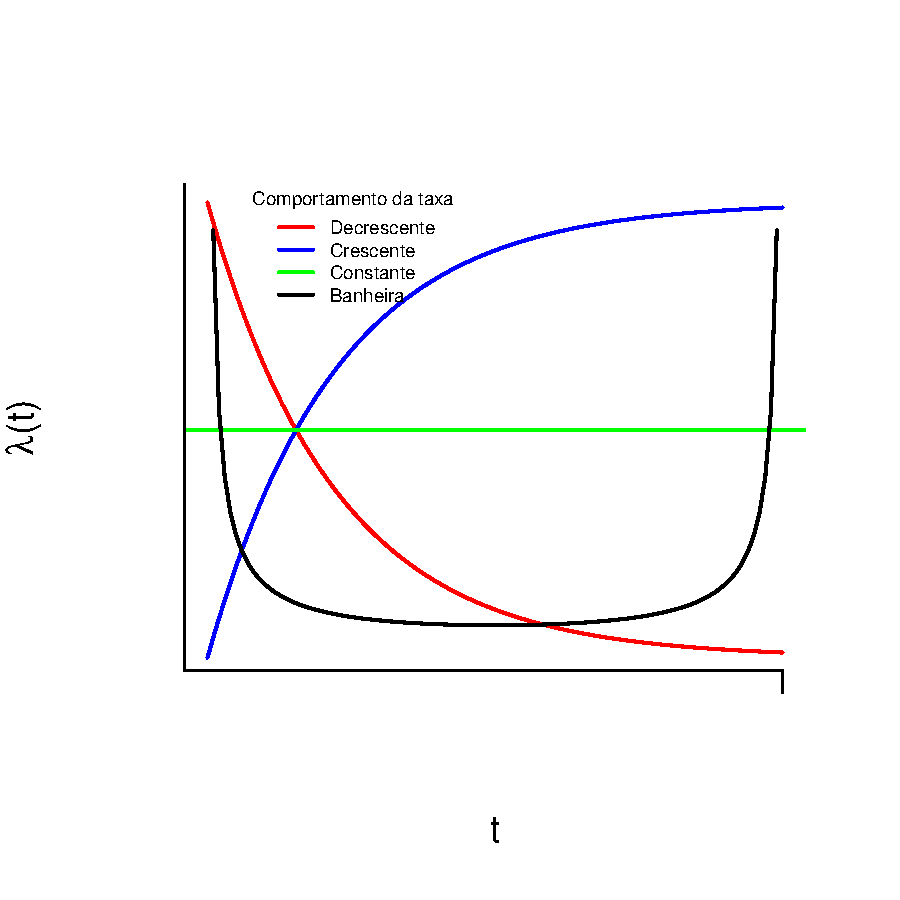
\includegraphics[height=8cm,width=10cm]{images/Graf_Risco.pdf}
  \vspace{-0.8cm}
  \caption{Diferentes comportamentos para $\mu(t)$}
  %% \label{Fig1}
  \centering
\end{figure}
\end{frame}
%%%-------------------------------------------------------------------
\begin{frame}{Processo de Poisson}
O Processo de Poisson configura um processo de contagem em que 
$Y(t),t\geqslant 0$, representa o número de eventos que ocorrem até $t$, 
satisfazendo:
\vspace{0,5cm}
\begin{enumerate}
  \item $Y(t)$ é inteiro e não negativo;
  \item Para $s<t$, $Y(s)\leq Y(t)$;
  \item $Y(t)-Y(s)$ é o número de eventos que ocorrem no intervalo $(s,t]$;
\item O processo é estacionário:

$$
  Y(t_{2}+s)-Y(t_{1}+s) \overset{i.d. }{\sim}Y(t_{2})-Y(t_{1}), \forall s>0
$$
  
\item O processo tem incrementos independentes, ou seja, os números de 
eventos verificados em intervalos disjuntos são independentes.
\end{enumerate}

\end{frame}

%%%-------------------------------------------------------------------
\begin{frame}{Diferentes padrões em processos de contagens}

\begin{figure}[h]
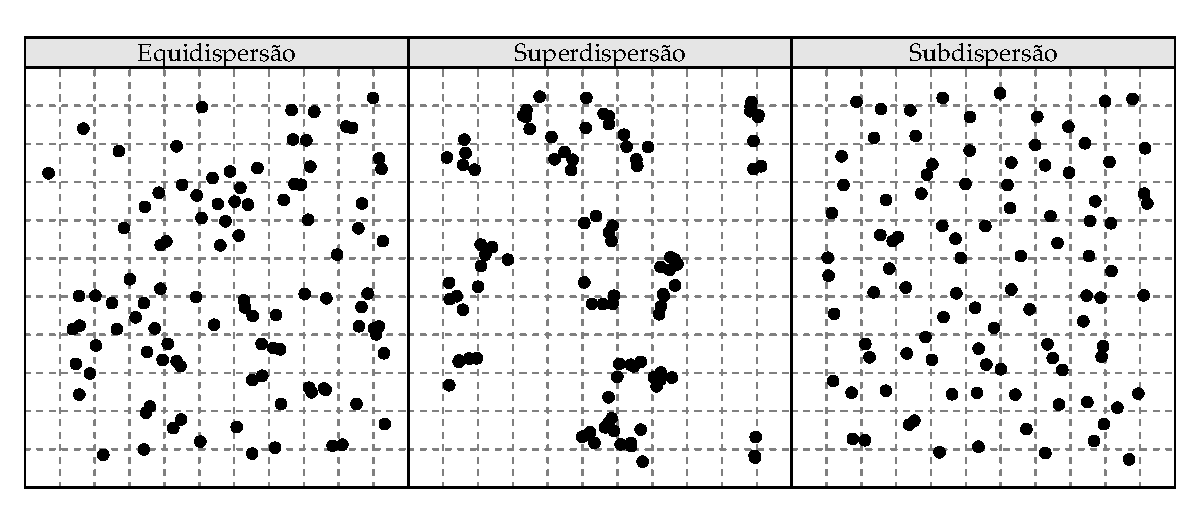
\includegraphics[scale=0.6]{images/processos14.pdf}
\caption{Ilustração de diferentes tipos de processos de contagens.}
\label{Fig2}
\centering

\end{figure}
\end{frame}

%%%-------------------------------------------------------------------
\begin{frame}{O desafio de dados de contagem}
\begin{itemize}
\item Poisson implica equidispersão, ou seja, $\mathrm{E}(Y) = \mathrm{var}(Y) = \mu. $
\vspace{0,5cm}
\item Na prática podemos ter
\begin{itemize}
  \item Subdispersão $\mathrm{E}(Y) > \mathrm{var}(Y)$;
  \item Superdispersão $\mathrm{E}(Y) < \mathrm{var}(Y)$.
\end{itemize}
\vspace{0,5cm}
  \item Desvios da equidispersão implicam: 
  \begin{itemize}
    \item Mais ou menos zeros e
    \item Caudas mais leves ou mais pesadas que o modelo Poisson.
  \end{itemize}
\end{itemize}
\end{frame}

%%%-------------------------------------------------------------------
\begin{frame}{Causas da não equidispersão}
\begin{itemize}
\item Desvios do processo Poisson;
\item Heterogeneidade entre unidades amostrais.
\vspace{0,5cm}
\item O que acontece caso o modelo Poisson seja usada para dados não equidispersos?
\begin{enumerate}
  \item Superdispersão: erros padrões associados aos coeficientes de 
  regressão serão subestimados.
  \item Subdispersão: erros padrões associados aos coeficientes de 
  regressão serão superestimados.
\end{enumerate}
\vspace{0,5cm}
  \item Ambos os casos o modelo Poisson resulta em erros padrões 
  não-confiáveis o que implica em inferências incorretas.
\end{itemize}
\end{frame}

%%%-------------------------------------------------------------------
\begin{frame}{Como lidar com a não equidispersão}
\begin{itemize}
\item Mudar a distribuição dos tempos entre eventos: Ex Gamma-Count. 
\vspace{0,5cm}
\item Incluir efeitos aleatórios ao nível das observações. Ex Poisson-Tweedie.
\vspace{0,5cm}
\item Modificar a distribuição de Poisson incluindo um parâmetro extra
de dispersão. Ex COM-Poisson.
\end{itemize}
\end{frame}

\section{Distribuições para contagens: propriedades e modelos de regressão}
\label{Section2}




\subsection{Distribuição Poisson}

%%%-------------------------------------------------------------------
\begin{frame}{Distribuição Poisson}
\begin{itemize}
\item Função de probabilidade
\begin{eqnarray}
f(y;\mu) &=& \frac{\mu^y}{y!}\exp\{-\mu\} \nonumber \\
	     &=& \frac{1}{y!} \exp \{\phi y -  \exp\{\phi\} \}, \quad y \in \mathbb{N}_{0},
\end{eqnarray}
onde $\phi = \log \{\mu\} \in \mathbb{R}$ e $\kappa(\phi) = \exp\{\phi\}$
denota a função cumulante.
\vspace{0,5cm}
\item $\mathrm{E}(Y) = \kappa^{\prime}(\phi) = \exp\{\phi\} = \mu$. 
\vspace{0,5cm}
\item $\mathrm{var}(Y) = \kappa^{\prime \prime}(\phi) = \exp\{\phi\} = \mu$.
\vspace{0,5cm}
\item Em \texttt{R} temos \texttt{dpois()}.

\end{itemize}
\end{frame}

%%%-------------------------------------------------------------------
\begin{frame}{Regressão Poisson}
\begin{itemize}
\item Considere $(y_i, x_i)$, $i = 1,\ldots, n$, onde $y_i$'s são iid 
realizações de $Y_i$ de acordo com a distribuição Poisson.
\vspace{0,5cm}
\item Modelo de regressão Poisson
$$Y_i \sim P(\mu_i), \quad  \text{sendo} \quad \mu_i = g^{-1}(\boldsymbol{x_i}^{\top} \boldsymbol{\beta}),$$
onde $\boldsymbol{x_i}$ and $\boldsymbol{\beta}$ são vetores $(p \times 1)$
de covariáveis conhecidas e parâmetros de regressão.
\vspace{0,5cm}
\item Em \texttt{R} temos \texttt{glm(..., family = poisson)}.
\vspace{0,5cm}
\item $g$ função de ligação (log link).
\end{itemize}
\end{frame}

%%%-------------------------------------------------------------------
\subsection{Distribuição Gamma-Count}

\begin{frame}
  \begin{center}
    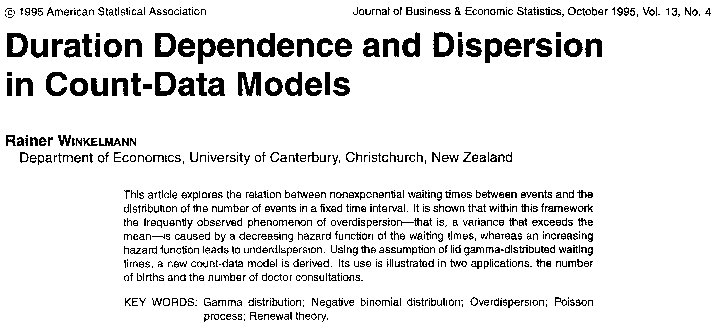
\includegraphics[width=11cm]{images/winkelman95.jpeg}
  \end{center}
  \begin{thebibliography}{99}
  \bibitem{Winkelmann1995}
    \MakeUppercase{Winkelmann, R.}
    \newblock{Duration Dependence and Dispersion in Count-Data Models}.
    \textbf{Journal of Business \& Economic Statistics}, v.13, n.4,
    p.467--474, 1995.
  \end{thebibliography}
\end{frame}

%%%-------------------------------------------------------------------
\begin{frame}
  \frametitle{Duração dependência}
  \begin{itemize}
  \item Considere um processo estocástico definido pela sequência da
    va $\tau_k$, intervalo de tempo entre eventos.
  \item Se $\{\tau_1, \tau_2,\ldots\}$ são independentes e identicamente
    distribuídos, todos com densidade $f(\tau)$, esse processo é chamado
    de \emph{renewal process}.
  \item Defina a variável de contagem $Y_T$ como o número de eventos no
    intervalo $[0,T)$.
  \item Defina $\vartheta_y = \sum_{k=1}^{y} \tau_k$ o tempo até o
    $y$-ésimo evento.
  \item A distribuição de $\vartheta_y$ determina a distribuição de
    $Y_T$, mas é baseada em convolução.
  \item São distribuições fechadas para convolução: normal, Poisson,
    binomial e gama.
  \item Destas, apenas a gama é contínua e positiva.
  \end{itemize}
\end{frame}

%%%-------------------------------------------------------------------
\begin{frame}[allowframebreaks]
  \frametitle{Relação entre número de eventos e intervalo entre eventos}
  \begin{itemize}
  \item Intervalos entre tempo $\tau_k \sim \text{G}(\alpha,\gamma)$,
  (omitindo $k$) temos
    $$f(\tau, \alpha, \gamma) = \frac{\gamma^\alpha}{\Gamma(\alpha)}
    \cdot \tau^{\alpha-1}\cdot \exp\{-\gamma\tau\},$$
    $$ \text{E}(\tau) = \frac{\alpha}{\gamma}, \quad
    \text{var}(\tau) = \frac{\alpha}{\gamma^2}.$$
  \item Tempo até o $y$-ésimo evento
    $$\vartheta_y = \tau_1+\cdots+\tau_y ~ \sim
    \text{G}(y\alpha, \gamma),$$
    $$f_y(\vartheta, \alpha, \gamma) =
    \frac{\gamma^{y\alpha}}{\Gamma(y\alpha)}\cdot
    \vartheta^{y\alpha-1}\cdot \exp\{-\gamma\vartheta\},$$
    $$ \text{E}(\vartheta) = \frac{y\alpha}{\gamma}, \quad
    \text{var}(\vartheta) = \frac{y\alpha}{\gamma^2}.$$

    \framebreak

  \item A distribuição acumulada do tempo até $\vartheta_{y}$ é
    $$F_y(T) = \Pr(\vartheta_y \leq T) = \int_{0}^{T}
    \frac{\gamma^{y\alpha}}{\Gamma(y\alpha)}\cdot t^{y\alpha-1}\cdot
    \exp\{-\gamma t\}\,\text{d}t.$$
  \item Seja $[0,T)$ um intervalo e $Y_{T}$ a va número de eventos
    neste intervalo.
  \item Segue que $Y_T < y$ se e somente se $\vartheta_y \geq
    T$. Assim
    $$\Pr(Y_T < y) = \Pr(\vartheta_y \geq T) = 1-F_y(T);$$
  \item Já que $\Pr(Y_T = y) = \Pr(Y_T < y+1) - \Pr(Y_T < y)$, então
    $$\Pr(Y_T = y) = F_y(T) - F_{y+1}(T).$$

    \framebreak

  \item Portanto, distribuição de $Y_T$ é resultado da diferença de
    acumuladas da distribuição Gama, 
    \begin{equation}
      F_y(T) = G(y\alpha, \gamma T) =
      \int_{0}^{T} \frac{\gamma^{y\alpha}}{\Gamma(y\alpha)}
      t^{y\alpha-1}\cdot\exp\{-\gamma t\}\, \text{d}t.
    \end{equation}
  \item Assim
    \begin{align*}
      \Pr(Y_T=y) &= G(y\alpha, \gamma T) - G((y+1)\alpha, \gamma T) \\
                 &= \left[ \int_{0}^{T}
                   \frac{\gamma^{y\alpha}}{\Gamma(y\alpha)}
                   t^{y\alpha-1}\cdot
                   \exp\{-\gamma t\}\, \text{d}t \right] \\
                 &\quad -
                   \left[ \int_{0}^{T}
                   \frac{\gamma^{(y+1)\alpha}}{\Gamma((y+1)\alpha)}
                   t^{(y+1)\alpha-1}\cdot
                   \exp\{-\gamma t\}\, \text{d}t \right].
    \end{align*}
  \end{itemize}
\end{frame}

%%%-------------------------------------------------------------------
\begin{frame}[fragile]
  \frametitle{Função de probabilidade}
  \begin{itemize}
  \item Em \texttt{R} temos

\begin{knitrout}
\definecolor{shadecolor}{rgb}{0.969, 0.969, 0.969}\color{fgcolor}\begin{kframe}
\begin{alltt}
\hlstd{dgc} \hlkwb{<-} \hlkwa{function}\hlstd{(}\hlkwc{y}\hlstd{,} \hlkwc{gamma}\hlstd{,} \hlkwc{alpha}\hlstd{,} \hlkwc{log} \hlstd{=} \hlnum{FALSE}\hlstd{) \{}
  \hlstd{p} \hlkwb{<-} \hlkwd{pgamma}\hlstd{(}\hlkwc{q} \hlstd{=} \hlnum{1}\hlstd{,}
              \hlkwc{shape} \hlstd{= y} \hlopt{*} \hlstd{alpha,}
              \hlkwc{rate} \hlstd{= alpha} \hlopt{*} \hlstd{gamma)} \hlopt{-}
    \hlkwd{pgamma}\hlstd{(}\hlkwc{q} \hlstd{=} \hlnum{1}\hlstd{,}
           \hlkwc{shape} \hlstd{= (y} \hlopt{+} \hlnum{1}\hlstd{)} \hlopt{*} \hlstd{alpha,}
           \hlkwc{rate} \hlstd{= alpha} \hlopt{*} \hlstd{gamma)}
  \hlkwa{if}\hlstd{(log} \hlopt{==} \hlnum{TRUE}\hlstd{) \{p} \hlkwb{<-} \hlkwd{log}\hlstd{(p)\}}
  \hlkwd{return}\hlstd{(p)}
\hlstd{\}}
\end{alltt}
\end{kframe}
\end{knitrout}

\end{itemize}
\end{frame}
%%%-------------------------------------------------------------------

%%%-------------------------------------------------------------------
\begin{frame}[fragile]
\begin{figure}[h]
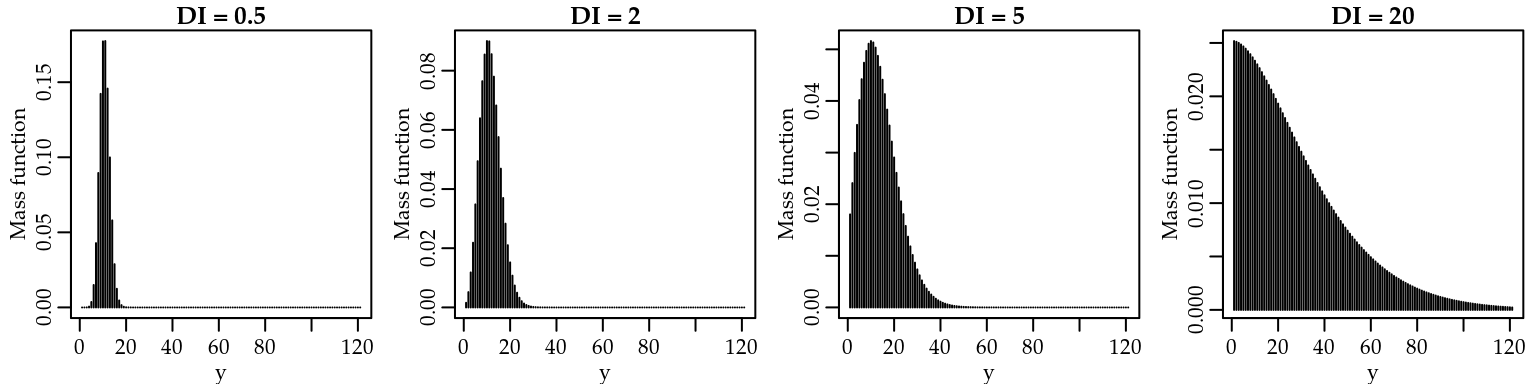
\includegraphics[scale=0.6]{images/GammaCount.png}
\caption{Função de probabilidade de acordo com valores do índice de dispersão - Gamma-Count.}
\label{Fig2}
\centering
\end{figure}
\begin{itemize}
\item Índice de dispersão - $\mathrm{DI} =  \mathrm{E}(Y)/\mathrm{var}(Y)$
\end{itemize}
\end{frame}

%%%-------------------------------------------------------------------
\begin{frame}[allowframebreaks]
  \frametitle{Parametrização para modelo de regressão}
  \begin{itemize}
  \item A média da variável aleatória $Y_T$ é resultado de
    \begin{align*}
      \mathrm{E}(Y_T) &= \sum_{i=0}^{\infty} i\cdot \Pr(i) \\
           &= \sum_{i=1}^{\infty} i\cdot \Pr(i)\\
           &= \sum_{i=1}^{\infty} G(i\alpha, \gamma T).\\
    \end{align*}
  \item Para um $T$ cada vez maior, tem-se que
    \begin{equation*}
      Y(T)\; \dot{\sim}\; \text{N}\left(
        \frac{\gamma}{\alpha},
        \frac{\gamma}{\alpha^2}\right).
    \end{equation*}
  \item Considere que
    $$\frac{\gamma}{\alpha} = \exp\{\boldsymbol{x}^{\top}\beta\} \Rightarrow
    \gamma = \alpha \exp\{\boldsymbol{x}^{\top}\beta\}.$$
    Essa parametrização produz um modelo de regressão para a média
    do tempo entre eventos definida por
    $$\text{E}(\tau|\boldsymbol{x}) = \frac{\alpha}{\gamma} =
    \exp\{-\boldsymbol{x}^{\top}\beta\}.$$
  \item O modelo de regressão é para o tempo entre eventos ($\tau$)
    e não diretamente para contagem porque, a menos que
    $\alpha = 1$, não é certo que
    $\text{E}(Y_i|x_i) = [\text{E}(\tau_i|x_i)]^{-1}$.
  \item $\alpha$ é um parâmetro de dispersão, assim $\alpha > 1$ indica
  subdispersão, $\alpha = 1$ equidispersão e $\alpha < 1$ superdispersão.
  \item Em \texttt{R} temos \texttt{MrDCR::gcnt(formula, data)}.
  \end{itemize}
  
\end{frame}
%%%-------------------------------------------------------------------

%%%-------------------------------------------------------------------
\subsection{Distribuição Poisson-Tweedie}

\begin{frame}[c]
\frametitle{Distribuição Tweedie}
\begin{itemize}
\item Distribuição Tweedie (J{\o}rgensen, 1997)
\begin{equation*}
\label{distri}
f(z; \mu, \phi, p) = a(z,\phi,p) \exp\{(z\psi - k(\psi))/\phi\},
\end{equation*}
onde $\mu = \mathrm{E}(Z) = k^{\prime}(\psi)$ é a média. 
\item $\phi > 0$ e $\psi$ são os parâmetros de dispersão e canônico.
\item $k(\psi)$ é a função cumulante e $a(z,\phi, p)$ é a constante normalizadora.
\item $\mathrm{var}(Z) = \phi \mu^p$ onde $p \in (-\infty  ,0] \cup [1,\infty)$ é 
um index determinando a distribuição.
\item Casos especiais: Normal ($p=0$), Poisson ($p=1$), não-central gamma ($p=1.5$), gamma ($p=2$), normal inversa ($p=3$) and distribuições estáveis ($p > 2$).
\item Notação $Z \sim Tw_p(\mu, \phi)$.
\end{itemize}
\end{frame}
%=======================================================================

%=======================================================================
\begin{frame}[c]
\frametitle{Distribuição Poisson-Tweedie}
\begin{itemize}
\item Especificação hierárquica:
\begin{align}
\begin{split}
\label{conditional}
Y|Z &\sim P(Z) \\ 
Z &\sim Tw_p(\mu, \phi). \nonumber
\end{split}
\end{align}
\item Função de probabilidade $(p > 1)$
\begin{equation*}
f(y;\mu,\phi,p) = \int_0^\infty \frac{z^y \exp^{-z}}{y!} a(z,\phi,p) \exp\{(z\psi - k(\psi))/\phi\} dz.
\end{equation*}
\item Forma fechada está disponível apenas no caso especial - binomial negativa ($p=2$).
\item Pode ser aproximada por integração Monte Carlo e/ou integração Gauss-Laguerre.
\end{itemize}
\end{frame}
%=======================================================================

%%%-------------------------------------------------------------------
\begin{frame}[fragile]
  \frametitle{Função de probabilidade}
  \begin{itemize}
  \item Em \texttt{R} temos

\begin{knitrout}
\definecolor{shadecolor}{rgb}{0.969, 0.969, 0.969}\color{fgcolor}\begin{kframe}
\begin{alltt}
\hlkwd{require}\hlstd{(tweedie)}
\hlcom{# Integrand Poisson X Tweedie distributions}
\hlstd{integrand} \hlkwb{<-} \hlkwa{function}\hlstd{(}\hlkwc{x}\hlstd{,} \hlkwc{y}\hlstd{,} \hlkwc{mu}\hlstd{,} \hlkwc{phi}\hlstd{,} \hlkwc{power}\hlstd{) \{}
    \hlstd{int} \hlkwb{=} \hlkwd{dpois}\hlstd{(y,} \hlkwc{lambda} \hlstd{= x)}\hlopt{*}\hlkwd{dtweedie}\hlstd{(x,} \hlkwc{mu} \hlstd{= mu,}
                                        \hlkwc{phi} \hlstd{= phi,} \hlkwc{power} \hlstd{= power)}
    \hlkwd{return}\hlstd{(int)}
\hlstd{\}}

\hlcom{# Computing the pmf using Monte Carlo}
\hlstd{dptw} \hlkwb{<-} \hlkwa{function}\hlstd{(}\hlkwc{y}\hlstd{,} \hlkwc{mu}\hlstd{,} \hlkwc{phi}\hlstd{,} \hlkwc{power}\hlstd{,} \hlkwc{control_sample}\hlstd{) \{}
    \hlstd{pts} \hlkwb{<-} \hlstd{control_sample}\hlopt{$}\hlstd{pts}
    \hlstd{norma} \hlkwb{<-} \hlstd{control_sample}\hlopt{$}\hlstd{norma}
    \hlstd{integral} \hlkwb{<-} \hlkwd{mean}\hlstd{(}\hlkwd{integrand}\hlstd{(pts,} \hlkwc{y} \hlstd{= y,} \hlkwc{mu} \hlstd{= mu,} \hlkwc{phi} \hlstd{= phi,}
                               \hlkwc{power} \hlstd{= power)}\hlopt{/}\hlstd{norma)}
    \hlkwd{return}\hlstd{(integral)}
\hlstd{\}}
\hlstd{dptw} \hlkwb{<-} \hlkwd{Vectorize}\hlstd{(dptw,} \hlkwc{vectorize.args} \hlstd{=} \hlstr{"y"}\hlstd{)}
\end{alltt}
\end{kframe}
\end{knitrout}

\end{itemize}
\end{frame}
%%%-------------------------------------------------------------------


%%%-------------------------------------------------------------------
\begin{frame}[fragile]
  \frametitle{Função de probabilidade}
  \begin{itemize}
  \item Exemplo

\begin{knitrout}
\definecolor{shadecolor}{rgb}{0.969, 0.969, 0.969}\color{fgcolor}\begin{kframe}
\begin{alltt}
\hlkwd{set.seed}\hlstd{(}\hlnum{123}\hlstd{)}
\hlstd{pts} \hlkwb{<-} \hlkwd{rtweedie}\hlstd{(}\hlkwc{n} \hlstd{=} \hlnum{1000}\hlstd{,} \hlkwc{mu} \hlstd{=} \hlnum{10}\hlstd{,} \hlkwc{phi} \hlstd{=} \hlnum{1}\hlstd{,} \hlkwc{power} \hlstd{=} \hlnum{2}\hlstd{)}
\hlstd{norma} \hlkwb{<-} \hlkwd{dtweedie}\hlstd{(pts,} \hlkwc{mu} \hlstd{=} \hlnum{10}\hlstd{,} \hlkwc{phi} \hlstd{=} \hlnum{1}\hlstd{,} \hlkwc{power} \hlstd{=} \hlnum{2}\hlstd{)}
\hlstd{control_sample} \hlkwb{<-} \hlkwd{list}\hlstd{(}\hlstr{"pts"} \hlstd{= pts,} \hlstr{"norma"} \hlstd{= norma)}
\hlkwd{dptw}\hlstd{(}\hlkwc{y} \hlstd{=} \hlkwd{c}\hlstd{(}\hlnum{0}\hlstd{,} \hlnum{5}\hlstd{,} \hlnum{10}\hlstd{,} \hlnum{15}\hlstd{),} \hlkwc{mu} \hlstd{=} \hlnum{10}\hlstd{,} \hlkwc{phi} \hlstd{=} \hlnum{1}\hlstd{,} \hlkwc{power} \hlstd{=} \hlnum{2}\hlstd{,}
     \hlkwc{control_sample} \hlstd{= control_sample)}
\end{alltt}
\begin{verbatim}
## [1] 0.09374152 0.05902132 0.03539478 0.02171625
\end{verbatim}
\begin{alltt}
\hlkwd{dnbinom}\hlstd{(}\hlkwc{x} \hlstd{=} \hlkwd{c}\hlstd{(}\hlnum{0}\hlstd{,} \hlnum{5}\hlstd{,} \hlnum{10}\hlstd{,} \hlnum{15}\hlstd{),} \hlkwc{mu} \hlstd{=} \hlnum{10}\hlstd{,} \hlkwc{size} \hlstd{=} \hlnum{1}\hlstd{)}
\end{alltt}
\begin{verbatim}
## [1] 0.09090909 0.05644739 0.03504939 0.02176291
\end{verbatim}
\end{kframe}
\end{knitrout}

\end{itemize}
\end{frame}
%%%-------------------------------------------------------------------

%=======================================================================
\begin{frame}[c]
\frametitle{Momentos e casos especiais}
\begin{itemize}
\item Média e variância marginal são facilmente obtidos
\begin{eqnarray}
\label{marginalGaussian}
\mathrm{E}(Y) &=& \mu \nonumber    \\
\mathrm{var}(Y) &=& \mu + \phi\mu^p. \nonumber
\end{eqnarray}
\item Casos especiais: Hermite ($p=0$), Neyman-Type A ($p=1$), 
      P\'olya-Aeppli ($p=1.5$), binomial negativa $(p=2)$ e Poisson inversa-Normal ($p=3$).
\item Cuidado! - Hermite é um caso limite.
\item $p$ é um índice que distingue entre importantes distribuições.
\item Espaço paramétrico de $p$ é não trivial $p \in {0}\cup[1,\infty)$.
\item Estimação de $p$ funciona como uma seleção automática de distribuições.
\item Notação $Y \sim PTw_p(\mu, \phi)$.
\end{itemize}
\end{frame}
%=======================================================================

%%%-------------------------------------------------------------------
\begin{frame}[fragile]
\begin{figure}[h]
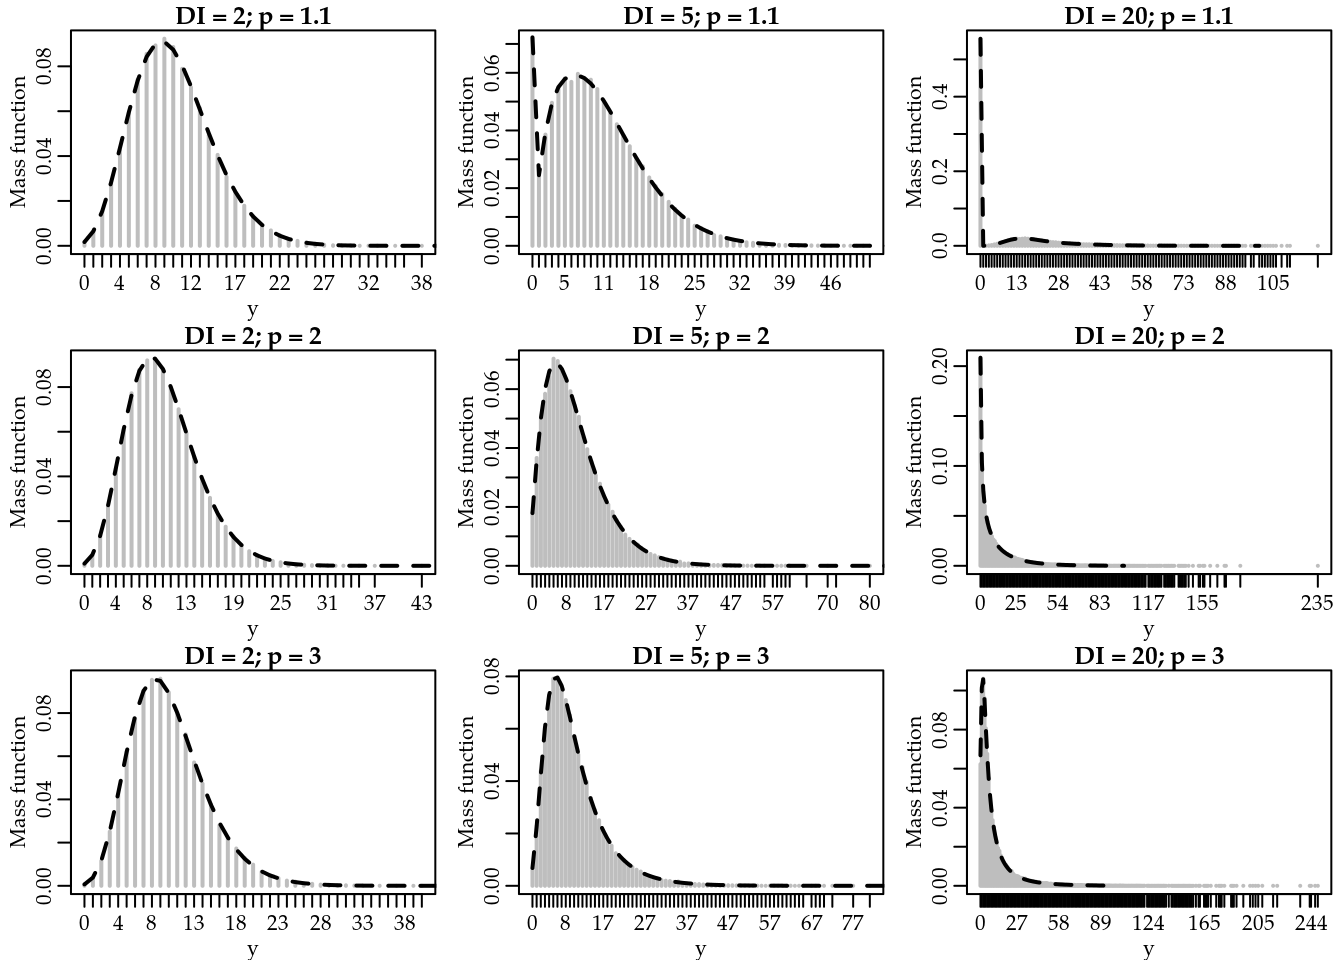
\includegraphics[scale=0.5]{images/PoissonTweedie.png}
\caption{Distribuição de probabilidade empírica (cinza) e função de 
probabilidade aproximada (preta) por valores do
índice de dispersão e valores do parâmetro de potência: Poisson-Tweedie.}
\label{Fig3}
\centering
\end{figure}
\end{frame}

%%%-------------------------------------------------------------------

%%%-------------------------------------------------------------------
\begin{frame}{Regressão Poisson-Tweedie}
\begin{itemize}
\item Considere $(y_i, x_i)$, $i = 1,\ldots, n$, onde $y_i$'s são iid 
realizações de $Y_i$ de acordo com a distribuição Poisson-Tweedie.
\vspace{0,5cm}
\item Modelo de regressão Poisson-Tweedie
$$Y_i \sim PTw_{p}(\mu_i, \phi), \quad  \text{sendo} \quad 
\mu_i = g^{-1}(\boldsymbol{x_i}^{\top} \boldsymbol{\beta}),$$
onde $\boldsymbol{x_i}$ and $\boldsymbol{\beta}$ são vetores $(p \times 1)$
de covariáveis conhecidas e parâmetros de regressão.
\vspace{0,5cm}
\item Em \texttt{R} temos \texttt{dptw()}.
\item $g$ função de ligação (log link).
\end{itemize}
\end{frame}

%%%-------------------------------------------------------------------
\subsection{Distribuição COM-Poisson}

\begin{frame}[allowframebreaks]{Distribuição COM-Poisson}

\begin{itemize}
    \item Nome COM-Poisson, advém de seus autores {\bf CO}nway e
    {\bf M}axwell (também é chamada de distribuição
    Conway-Maxwell-Poisson).
    \item Proposta em um contexto de filas,
    essa distribuição generaliza a Poisson com a adição de um parâmetro.
    \item Modifica a relação entre probabilidades consecutivas.
    \begin{multicols}{2}
        \begin{itemize}
            \item {\bf Distribuição Poisson}\\
            $$\frac{Pr(Y = y-1)}{Pr(Y = y)} = \frac{y}{\lambda}$$
            \item {\bf Distribuição COM-Poisson}\\
            $$\frac{Pr(Y = y-1)}{Pr(Y = y)} = \frac{y^\nu}{\lambda}$$
        \end{itemize}
    \end{multicols}   
\end{itemize}

\framebreak

\begin{block}{Distribuição de probabilidades}
\begin{center}
\begin{equation*} 
    f(y; \lambda, \nu) = \frac{\lambda^y}{(y!)^\nu 
    Z(\lambda, \nu)}, \quad \textrm{em que }\, Z(\lambda, \nu) = 
    \sum_{j=0}^\infty \frac{\lambda^j}{(j!)^\nu} \textrm{; e}\quad
    \lambda > 0, \, \nu \geq 0
\end{equation*}
\end{center}
\end{block}

\begin{block}{Casos particulares}
\begin{itemize}
	\item Distribuição Poisson, quando $\nu = 1$
	\item Distribuição Bernoulli, quando $\nu \rightarrow \infty$
	\item Distribuição Geométrica, quando $\nu = 0, \quad \lambda < 1$
\end{itemize}
\end{block}
\end{frame}

%%%-------------------------------------------------------------------
\begin{frame}{Distribuição COM-Poisson}

\begin{columns}[t]
\begin{column}{.3\textwidth}
  \vspace{1cm}
    \begin{itemize}
      \setbeamercovered{transparent=35}
      \uncover<1>{\item Poisson $\nu = 1$}
      \uncover<2>{\item Bernoulli $\nu \rightarrow \infty$}
      \uncover<3>{\item Geométrica $\nu = 0,\, \lambda < 1$}
    \end{itemize}
  \vspace{1cm}
\end{column}

\begin{column}{.7\textwidth}
  \vspace{0.5cm}
  \only<1>{
  \vspace{-1.1cm}
  
\begin{knitrout}
\definecolor{shadecolor}{rgb}{0.969, 0.969, 0.969}\color{fgcolor}

{\centering 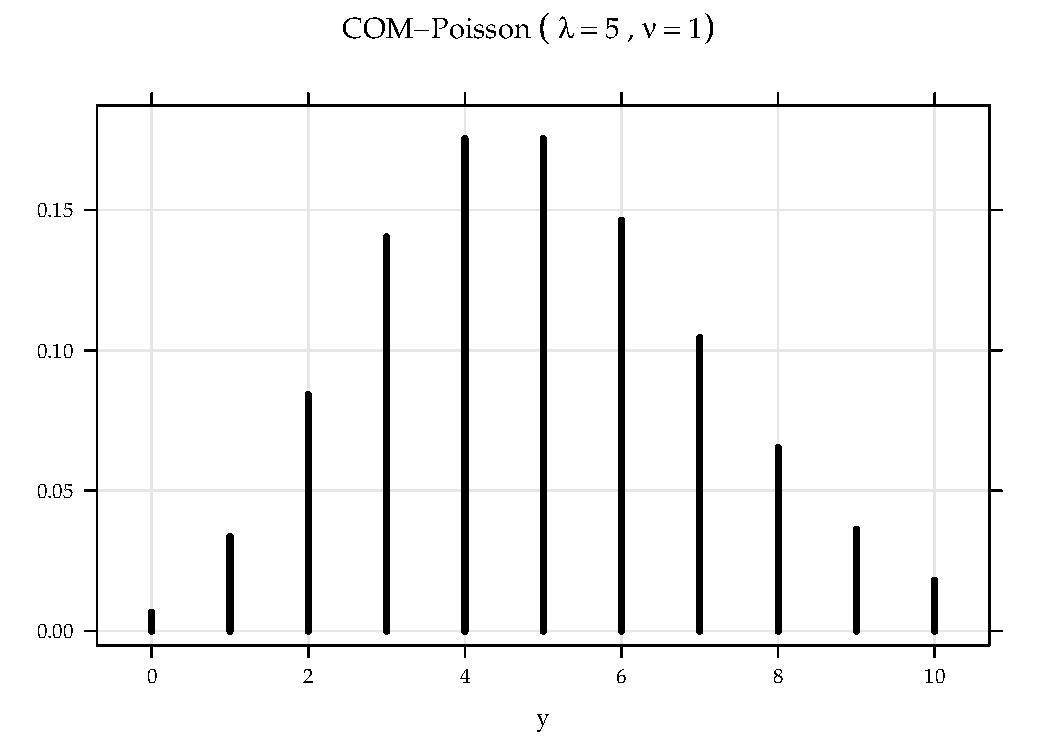
\includegraphics[width=0.9\textwidth]{figure/unnamed-chunk-4-1} 

}



\end{knitrout}
}
  \only<2>{
  \vspace{-1.1cm}
\begin{knitrout}
\definecolor{shadecolor}{rgb}{0.969, 0.969, 0.969}\color{fgcolor}

{\centering 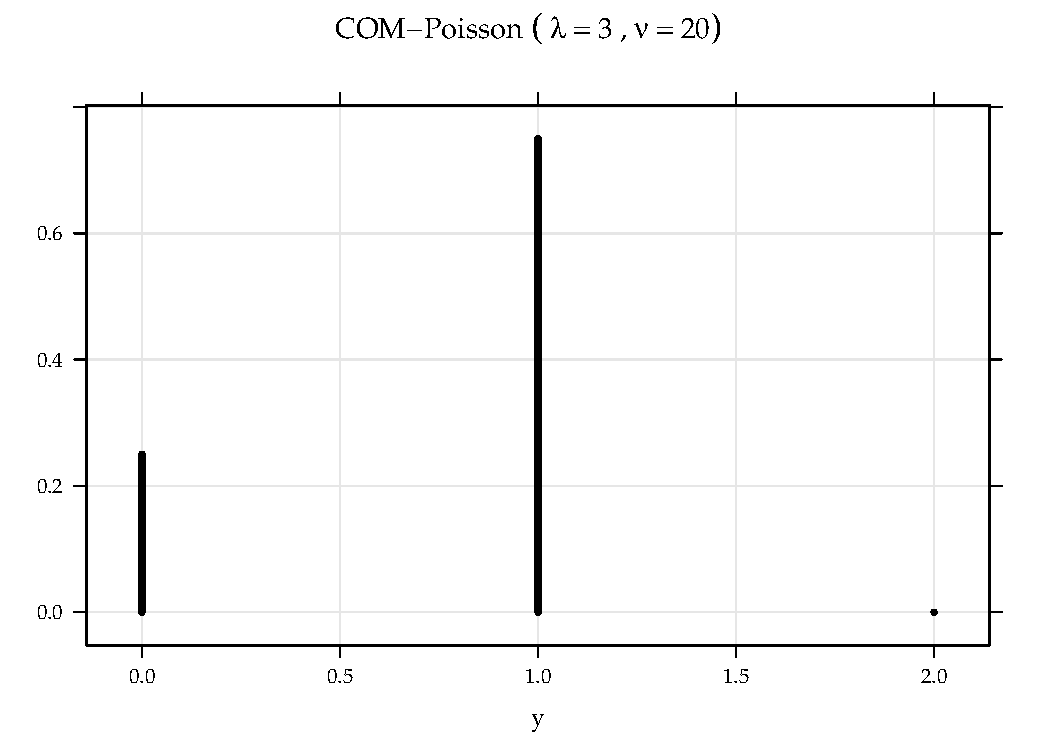
\includegraphics[width=0.9\textwidth]{figure/unnamed-chunk-5-1} 

}



\end{knitrout}
}
  \only<3>{
    \vspace{-1.1cm}
\begin{knitrout}
\definecolor{shadecolor}{rgb}{0.969, 0.969, 0.969}\color{fgcolor}

{\centering 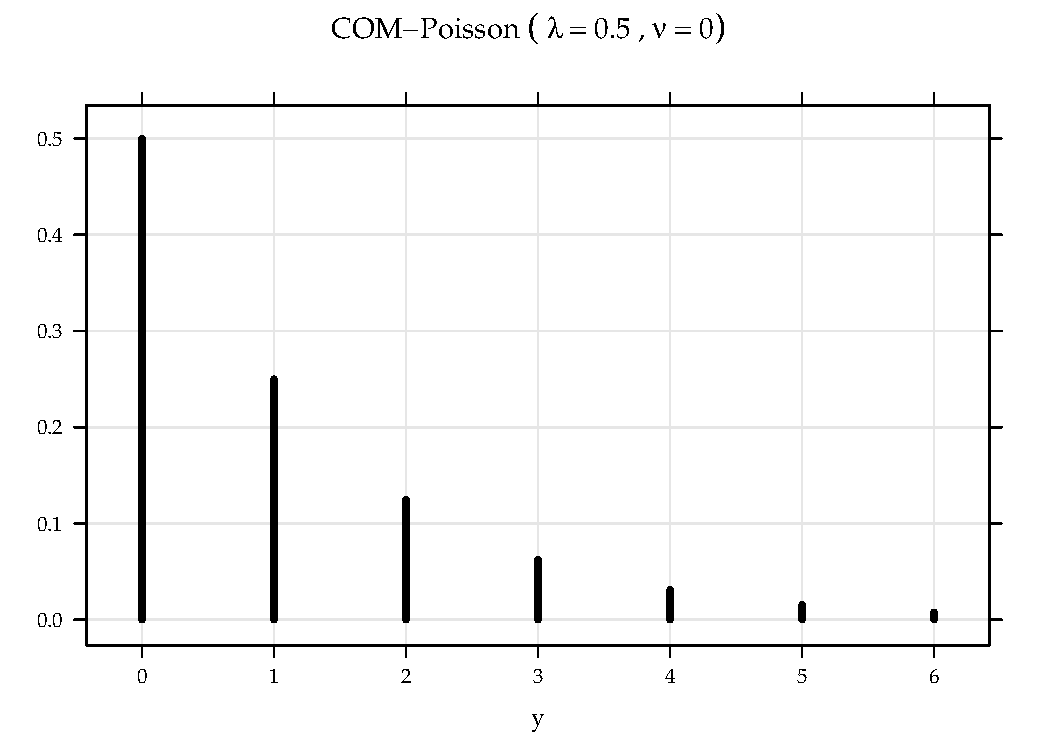
\includegraphics[width=0.9\textwidth]{figure/unnamed-chunk-6-1} 

}



\end{knitrout}
}
  \end{column}
\end{columns}

\end{frame}


%%%-------------------------------------------------------------------
\begin{frame}[fragile]
\begin{figure}[h]
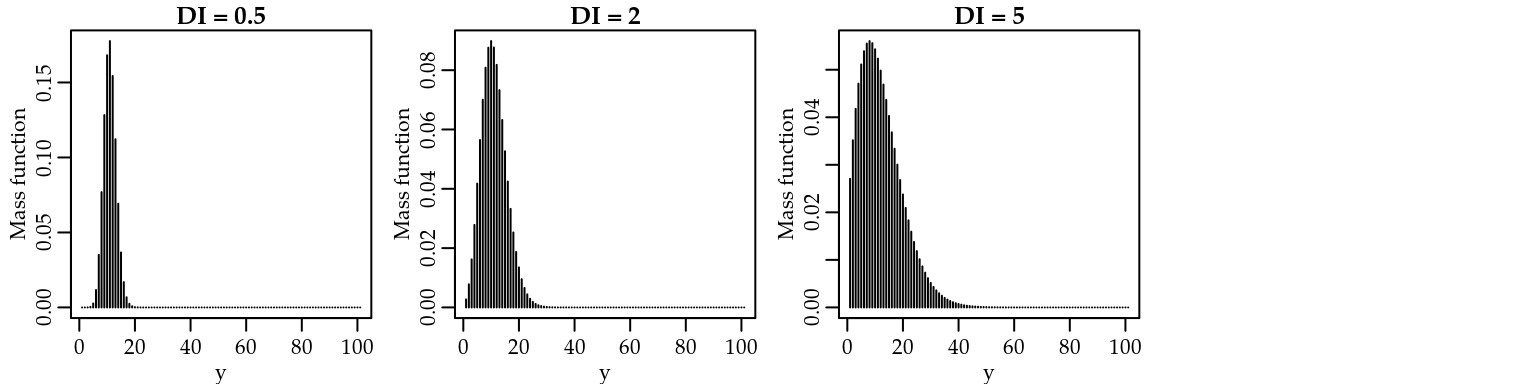
\includegraphics[scale=0.8]{images/COMPoisson.png}
\caption{Distribuição de probabilidade por valores do
índice de dispersão: COM-Poisson.}
\label{Fig3}
\centering
\end{figure}
\end{frame}

%%%-------------------------------------------------------------------
\begin{frame}{Assintocidade da função Z}

$$ Z(\lambda, \nu) = \sum_{j=0}^\infty \frac{\lambda^j}{(j!)^\nu} $$

\begin{knitrout}
\definecolor{shadecolor}{rgb}{0.969, 0.969, 0.969}\color{fgcolor}

{\centering 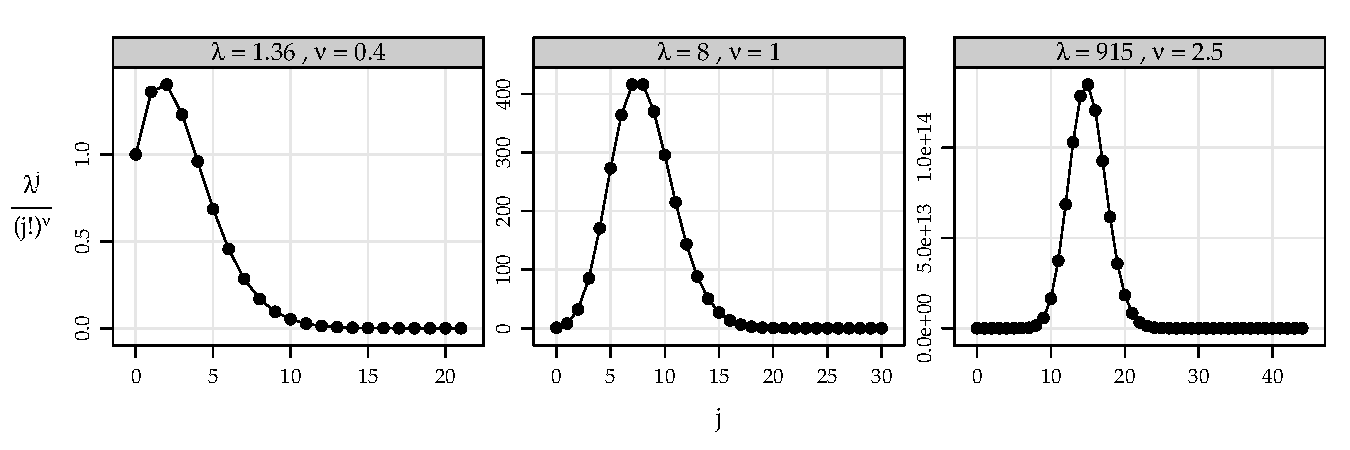
\includegraphics[width=1\textwidth]{figure/unnamed-chunk-7-1} 

}



\end{knitrout}
\end{frame}


%%%-------------------------------------------------------------------
\begin{frame}{Momentos da distribuição}

\begin{columns}[t,onlytextwidth]
\column{.48\textwidth}
Não tem expressão analítica, calculamos utilizando a definição de média e
variância;
\begin{itemize}
  \itemsep7.5pt\parskip0pt\parsep0pt
  \item $\mathrm{E}(Y) = \begin{aligned} 
            &\sum_{y = 0}^{\infty} y \cdot p(y)&
        \end{aligned}
        $
  \item $\mathrm{var}(Y) = \begin{aligned} 
            &\sum_{y = 0}^{\infty} y^2 \cdot p(y) - \mathrm{E}^2(Y)&
        \end{aligned}
        $
\end{itemize}

\column{.48\textwidth}
Aproximação proposta por Shimueli (2005), boa aproximação para $\nu 
\leq 1$ ou $\lambda > 10^\nu$ \\[0.2cm]
\begin{itemize}
  \itemsep7.5pt\parskip0pt\parsep0pt
  \item $\mathrm{E}(Y) \approx$ $\begin{aligned} 
            &\lambda ^ \frac{1}{\nu} - \frac{\nu - 1}{2\nu}&
        \end{aligned}
        $ 
  \item $\mathrm{var}(Y) \approx$ $\begin{aligned} 
            &\frac{1}{\nu}\cdot \mathrm{E}(Y)&
        \end{aligned}
        $
\end{itemize}
\end{columns}
\begin{itemize}
  \item Regressão COM-Poisson: $\lambda_i = \exp(\boldsymbol{x}_i^{\top} \boldsymbol{\beta})$, 
  em que $\boldsymbol{x}_i$ é o vetor de covariáveis do i-ésimo indivíduo e 
  $\boldsymbol{\beta}$ o vetor de parâmetros.
\end{itemize}
\end{frame}

%%%-------------------------------------------------------------------
\subsection{Comparando distribuições para contagens}
\begin{frame}{Medindo propriedades das distribuições}
\begin{itemize}

\item Índice de dispersão: $$\mathrm{DI} = \frac{\mathrm{var}(Y)}{\mathrm{E}(Y)}.$$
$ DI < 1$ subdispersão, $DI = 1$ equidispersão e $DI > 1$ superdispersão.
\vspace{0,5cm}
\item Índice de inflação de zeros: $$\mathrm{ZI} = 1 + \frac{\log \mathrm{P}(Y = 0)}{\mathrm{E}(Y)}.$$
$ZI < 0$ zero deflacionado, $ZI=1$ não zero inflacionado e $ZI > 1$ zero inflacionado.
\vspace{0,5cm}
\item Índice de cauda pesada:
$$ \mathrm{HT} = \frac{\mathrm{P}(Y=y+1)}{\mathrm{P}(Y=y)}\quad \text{for} \quad y \to \infty.$$
$\mathrm{HT} \to 1$ quando $y \to \infty$ indica cauda pesada.
\end{itemize}
\end{frame}

%%%-------------------------------------------------------------------
\begin{frame}[fragile]
\begin{figure}[h]
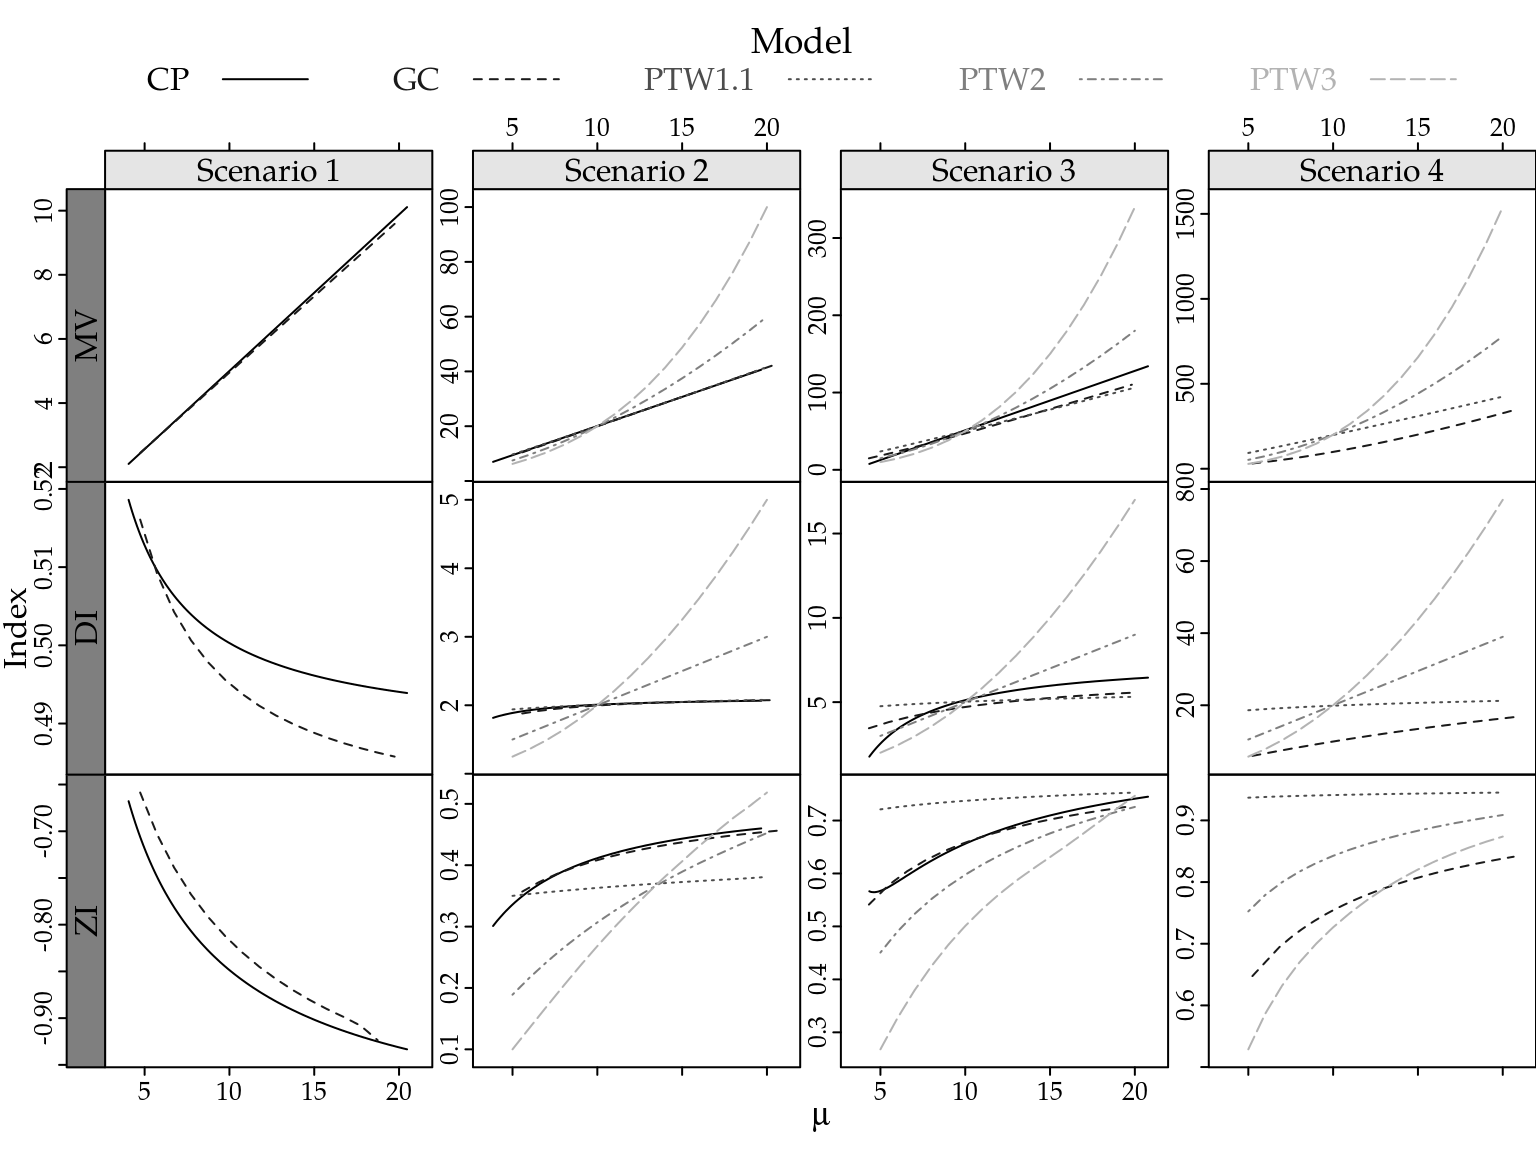
\includegraphics[scale=0.5]{images/Compara.png}
\caption{}
\label{Fig3}
\centering
\end{figure}
\end{frame}

%%%-------------------------------------------------------------------

%%%-------------------------------------------------------------------
\begin{frame}[fragile]
\begin{figure}[h]
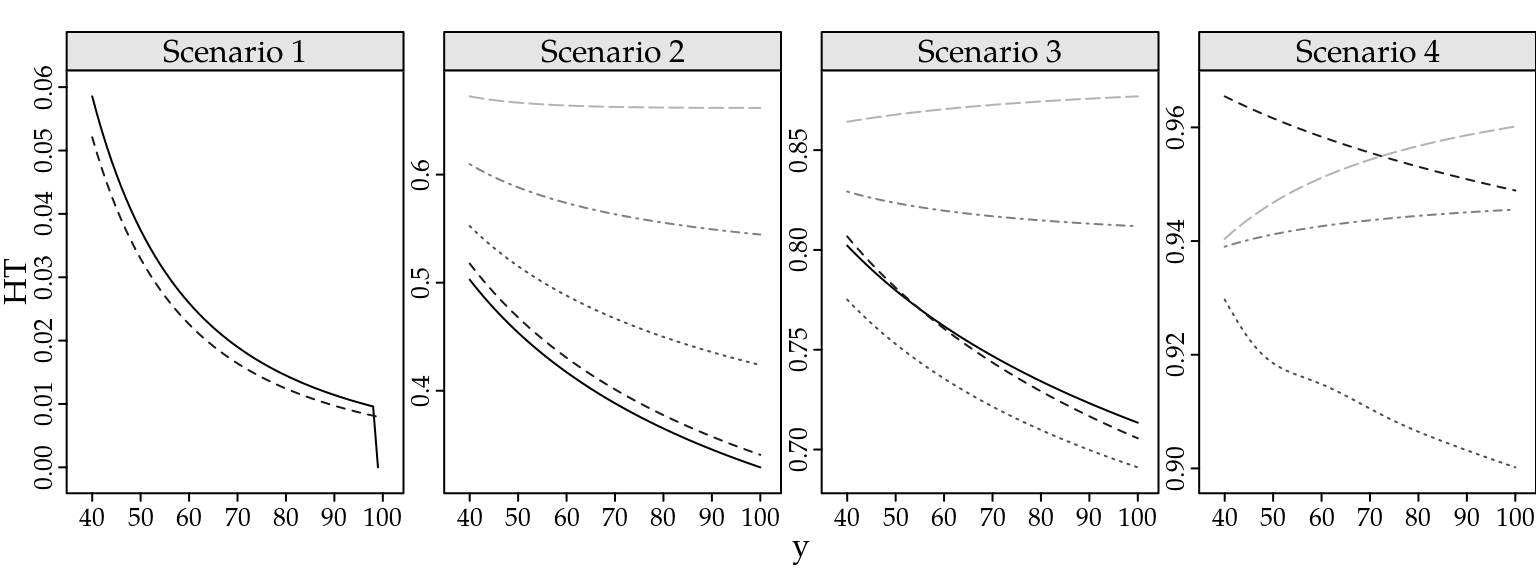
\includegraphics[scale=0.6]{images/heavytail-1.png}
\caption{Índice de cauda pesada para alguns valores extremos da va $Y$.}
\label{Fig3}
\centering
\end{figure}
\end{frame}

%%%-------------------------------------------------------------------

%%%-------------------------------------------------------------------
\begin{frame}[fragile]{Flexibilidade}
\begin{table}[h]
\centering
\caption{Reference models and dominant features by dispersion and power parameter values.}
\label{tab:model}
\begin{tabular}{llll} \hline
Modelo de referência     & Fatos dominantes                     & Dispersão           & Power   \\ \hline
Poisson                  & Equi                                 & $-$          & $-$      \\
Gamma-Count              & Sub, Equi, Super, deflação de zero   & $\alpha \lessgtr 1$ & $-$ \\
COM-Poisson              & Sub, Equi, Super, deflação de zero   & $\nu \lessgtr 1$    & $-$ \\
Hermite                  & Super                                & $\phi > 0$    & $p = 0$   \\
Neyman Type A            & Super, Zero-inflacionado             & $\phi > 0$          & $p = 1$ \\
\textit{Poisson compound Poisson} & Super, Zero-inflacionado    & $\phi > 0$ & $1 < p < 2$ \\
P\'olya-Aeppli           & Super, Zero-inflacionado             & $\phi > 0$ & $p = 1.5$ \\
Negative binomial        & Super                                & $\phi > 0$ & $p = 2$ \\
\textit{Poisson positive stable}  & Super, cauda pesada         & $\phi > 0$       & $p > 2$ \\
Poisson-inverse Gaussian & Super, cauda pesada                  & $\phi > 0$       & $p = 3$ \\ \hline
\end{tabular}
\end{table}
\end{frame}

%%%-------------------------------------------------------------------

\section{Método de máxima verossimilhança}
\label{Section3}




%%%-------------------------------------------------------------------
\begin{frame}{Método de máxima verossimilhança}
\begin{itemize}
  \item Conhecemos a distribuição que gerou os dados $f(y;\boldsymbol{\theta})$.
  \item Mas não seu finito vetor de parâmetros $\boldsymbol{\theta} \in \Theta$.
  \item $\Theta$ em geral é um subconjunto do $\mathbb{R}^n$.
  \item Dado $y$ uma observação da va $Y$ a função de verossimilhança 
  $$ L(\boldsymbol{\theta};y) = f(y;\boldsymbol{\theta}). $$
  \item Note que $f(y;\boldsymbol{\theta})$ é uma função de probabilidade
  no espaço amostral.
  \item Porém, $L(\boldsymbol{\theta};y) = f(y;\boldsymbol{\theta})$
  é uma função no espaço paramétrico $\Theta$.
  \item $L(\boldsymbol{\theta};y)$ expressa a plausibilidade para
  diferentes valores dos parâmetros após observarmos $y$ sem ter nenhuma
  outra informação sobre $\boldsymbol{\theta}$.
  \item Para dados de contagem a verossimilhança é a probabilidade de
  observar o ponto $y$ caso $\boldsymbol{\theta}$ seja o verdadeiro
  valor do parâmetro.
\end{itemize}
\end{frame}

%%%-------------------------------------------------------------------
\begin{frame}{Estimador de máxima verossimilhança}
\begin{itemize}
  \item Estimador de máxima verossimilhança (MLE) $L(\hat{\boldsymbol{\theta}}(y);y) = \underset{\boldsymbol{\theta}\in \Theta}\max L(\boldsymbol{\theta};y).$
  \item Seja $Y_i$ iid va com fp $f(y;\boldsymbol{\theta})$ então
  $$L(\boldsymbol{\theta};\boldsymbol{y}) = \prod_{i=1}^n L(\boldsymbol{\theta}; y_i) = \prod_{i=1}^n f(y_i; \boldsymbol{\theta}).$$
  \item Log-verossimilhança
  $$\ell(\boldsymbol{\theta})=\sum^n_{i=1} \log\{ L(\boldsymbol{\theta}; y_i) \}.$$
\end{itemize}
\end{frame}

%%%-------------------------------------------------------------------
\begin{frame}{Estimador de máxima verossimilhança}
\begin{itemize}
  \item MLE em geral pode ser obtido como a solução das equações de verossimilhança (ou escore)
  $$\mathcal{U}(\boldsymbol{\theta}) = \left ( \frac{\partial \ell(\boldsymbol{\theta})}{\partial \theta_1}^\top, \ldots, \frac{\partial \ell(\boldsymbol{\theta})}{\partial \theta_p}^\top \right )^\top = \boldsymbol{0}.$$
  \item Soluções analíticas são raras e métodos numéricos são necessários.
  \item A entrada $(i,j)$ da matrix $p \times p$ de informação de Fisher 
  $\mathcal{F}_{\boldsymbol{\theta}}$ para o vetor $\boldsymbol{\theta}$ é dada por
$$
\mathcal{F}_{\boldsymbol{\theta}_{ij}} =-\mathrm{E} \left \{ \frac{\partial^2 \ell(\boldsymbol{\theta})}{\partial\theta_i\partial\theta_j} \right \}.
$$
  \item Algorithm Newton scoring
$$  
\boldsymbol{\theta}^{(i+1)} = \boldsymbol{\theta}^{(i)} - \mathcal{F}_{\boldsymbol{\theta}}^{-1} \mathcal{U}(\boldsymbol{\theta}^{(i)}).
$$
  \item Distribuição assintótica $\boldsymbol{\hat{\theta}} \sim \mathrm{N}(\boldsymbol{\theta}, \mathcal{F}_{\boldsymbol{\theta}}^{-1})$.
\end{itemize}
\end{frame}

%%%-------------------------------------------------------------------
\begin{frame}{Comentários MLE}
\begin{itemize}
  \item A verdadeira distribuição que gerou os dados é conhecida.
  \item É possível obter de forma analítica a primeira e segunda derivada
  da log-verossimilhança.
  \item A log-verossimilhança é
  \begin{enumerate}
    \item Poisson sem problemas!
    \item Count-Gamma: diferença de duas integrais.
    \item Poisson-Tweedie: expressa como uma integral sem solução analítica.
    \item COM-Poisson: envolve uma soma infinita.
  \end{enumerate}
  \item Nestes casos não é possível obter expressões fechadas para as
  funções escore e matriz de informação de Fisher.
  \item Solução! Maximizar diretamente a log-verossimilhança usando
  algum método quase-Newton ou derivadas-free. 
  \item Exemplos BFGS, Gradiente conjugado, Nelder-Mead.
  \item Ver função \texttt{optim()} em \texttt{R}.
  
\end{itemize}
\end{frame}

%%%-------------------------------------------------------------------
\begin{frame}[fragile]{Exemplo: MLE distribuição Count-Gamma}
\begin{itemize}
  \item Log-verossimilhança
\begin{knitrout}
\definecolor{shadecolor}{rgb}{0.969, 0.969, 0.969}\color{fgcolor}\begin{kframe}
\begin{alltt}
\hlcom{# Função de probabilidade}
\hlstd{dgc} \hlkwb{<-} \hlkwa{function}\hlstd{(}\hlkwc{y}\hlstd{,} \hlkwc{gamma}\hlstd{,} \hlkwc{alpha}\hlstd{,} \hlkwc{log} \hlstd{=} \hlnum{FALSE}\hlstd{) \{}
  \hlstd{p} \hlkwb{<-} \hlkwd{pgamma}\hlstd{(}\hlkwc{q} \hlstd{=} \hlnum{1}\hlstd{,}
              \hlkwc{shape} \hlstd{= y} \hlopt{*} \hlstd{alpha,}
              \hlkwc{rate} \hlstd{= alpha} \hlopt{*} \hlstd{gamma)} \hlopt{-}
    \hlkwd{pgamma}\hlstd{(}\hlkwc{q} \hlstd{=} \hlnum{1}\hlstd{,}
           \hlkwc{shape} \hlstd{= (y} \hlopt{+} \hlnum{1}\hlstd{)} \hlopt{*} \hlstd{alpha,}
           \hlkwc{rate} \hlstd{= alpha} \hlopt{*} \hlstd{gamma)}
  \hlkwa{if}\hlstd{(log} \hlopt{==} \hlnum{TRUE}\hlstd{) \{p} \hlkwb{<-} \hlkwd{log}\hlstd{(p)\}}
  \hlkwd{return}\hlstd{(p)}
\hlstd{\}}
\hlcom{# Função de log-verossimilhança}
\hlstd{ll_gc} \hlkwb{<-} \hlkwa{function}\hlstd{(}\hlkwc{gamma}\hlstd{,} \hlkwc{alpha}\hlstd{,} \hlkwc{y}\hlstd{) \{}
  \hlstd{ll} \hlkwb{<-} \hlkwd{sum}\hlstd{(}\hlkwd{dgc}\hlstd{(}\hlkwc{y} \hlstd{= y,} \hlkwc{gamma} \hlstd{= gamma,} \hlkwc{alpha} \hlstd{= alpha,} \hlkwc{log} \hlstd{=} \hlnum{TRUE}\hlstd{))}
  \hlkwd{return}\hlstd{(}\hlopt{-}\hlstd{ll)}
\hlstd{\}}
\end{alltt}
\end{kframe}
\end{knitrout}

\end{itemize}
\end{frame}

%%%-------------------------------------------------------------------
\begin{frame}[fragile]{Exemplo: MLE distribuição Count-Gamma}
\begin{itemize}
  \item Maximização numérica e ajuste final
\begin{knitrout}
\definecolor{shadecolor}{rgb}{0.969, 0.969, 0.969}\color{fgcolor}\begin{kframe}
\begin{alltt}
\hlkwd{require}\hlstd{(bbmle)}
\hlstd{y} \hlkwb{<-} \hlkwd{rpois}\hlstd{(}\hlnum{100}\hlstd{,} \hlkwc{lambda} \hlstd{=} \hlnum{10}\hlstd{)}
\hlstd{fit_gc} \hlkwb{<-} \hlkwd{mle2}\hlstd{(ll_gc,} \hlkwc{start} \hlstd{=} \hlkwd{list}\hlstd{(}\hlstr{"gamma"} \hlstd{=} \hlnum{10}\hlstd{,} \hlstr{"alpha"} \hlstd{=} \hlnum{1}\hlstd{),}
               \hlkwc{data} \hlstd{=} \hlkwd{list}\hlstd{(}\hlstr{"y"} \hlstd{= y))}
\hlstd{fit_gc}
\end{alltt}
\begin{verbatim}
## 
## Call:
## mle2(minuslogl = ll_gc, start = list(gamma = 10, alpha = 1), 
##     data = list(y = y))
## 
## Coefficients:
##     gamma     alpha 
## 9.5321032 0.8224768 
## 
## Log-likelihood: -263.21
\end{verbatim}
\end{kframe}
\end{knitrout}

\end{itemize}
\end{frame}

\section{Modelos especificados por suposições de momentos}
\label{Section4}




\subsection{Especificação}
%%%-------------------------------------------------------------------
\begin{frame}{Motivação}
\begin{itemize}
  \item Assumem que a distribuição de probabilidade é completamente
  conhecida a menos de um vetor de parâmetros.
  \item Na prática pode ser difícil escolher uma particular distribuição.
  \item Difícil de estimar usando métodos baseados em verossimilhança.
  \item Nem sempre a esperança é conhecida.
  \item O efeito das covariáveis não são diretamente relacionados a esperança da va.
  \item Abordagem mais geral que se adapte automaticamente a estrutura de dispersão dos dados.
  \item Fácil de implementar.
  \item SOLUÇÃO: Poisson-Tweedie estendida.
\end{itemize}
\end{frame}

%%%-------------------------------------------------------------------
\begin{frame}[c]
\frametitle{Modelos de regressão}
\begin{itemize}
\item Considere $(y_i, \boldsymbol{x}_i)$, $i = 1, \ldots, n$, onde
$y_i$'s são iid. va's.
\item Especificação paramétrica completa: $$Y_i \sim \mathrm{PTw_p}(\mu_i, \phi).$$
\item Especificação baseada em momentos:
\begin{eqnarray}
\label{marginalGaussian}
\mathrm{E}(Y_i) &=& \mu_i \nonumber    \\
\mathrm{var}(Y_i) &=& \mu_i + \phi\mu_i^p \nonumber
\end{eqnarray}
onde $g(\mu_i) = \eta_i = \boldsymbol{x}_i^{\top} \boldsymbol{\beta}$,
$\boldsymbol{x}_i$ e $\boldsymbol{\beta}$ são ($p \times 1$) vetores
de covariáveis conhecidas e parâmetros de regressão desconhecidos.
\item $\mathrm{var}(Y_i) > 0$, assim $\phi > - \mu^{(1-p)}_i$ $\Longrightarrow$ sub, equi e superdispersão.
\item $g$ função de ligação (log link).
\end{itemize}
\end{frame}
%=======================================================================

%=======================================================================
\begin{frame}[c]
\frametitle{Modelos de regressão}
\begin{itemize}
\item Poisson-Tweedie estendida pode lidar com subdispersão $\phi < 0$.
\begin{figure}[h]
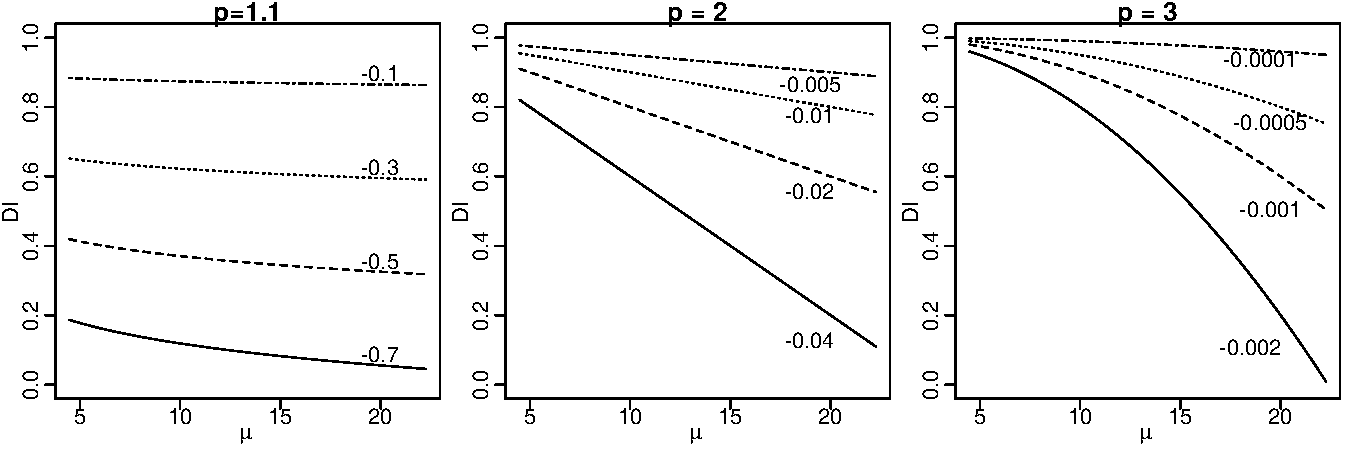
\includegraphics[scale=0.4]{images/Rplot.pdf}
\caption{\tiny{Índice de dispersão como uma função da média por valores dos parâmetros de dispersão e potência.}}
\label{SUBPTW}
\centering
\end{figure}
\item Máxima verossimilhança precisa da especificação paramétrica completa.
\item Funções de estimação (Bonat, et. al. 2016)
\item Espaço paramétrico para o parâmetro de potência é livre ($p \in \Re$).
\end{itemize}
\end{frame}
%=======================================================================

%=======================================================================
\subsection{Estimação e Inferência}
\begin{frame}[c]
\frametitle{Parâmetros de regressão}
\begin{itemize}
\item Seja $\boldsymbol{\theta} = (\boldsymbol{\beta}^\top, \boldsymbol{\lambda}^\top = (\phi, p)^\top)^\top$ 
o vetor de parâmetros.
\item Função quasi-score para os parâmetros de regressão
\begin{equation*}
\psi_{\boldsymbol{\beta}}(\boldsymbol{\beta}, \boldsymbol{\lambda}) = \left (\sum_{i=1}^n \frac{\partial \mu_i}{\partial \beta_1}C^{-1}_i(y_i - \mu_i)^\top, \ldots, \sum_{i=1}^n \frac{\partial \mu_i}{\partial \beta_Q}C^{-1}_i(y_i - \mu_i)^\top  \right )^\top,
\end{equation*}
onde $C_i = \mu_i + \phi \mu_i^p$ e $\partial \mu_i/\partial \beta_j = \mu_i x_{ij}$ para $j = 1, \ldots, p$.
\item A entrada $(j,k)$ da matriz $p \times p$ de sensitividade para $\psi_{\boldsymbol{\beta}}$ é dada por
\begin{equation}
\label{Sbeta}
\mathrm{S}_{\beta_{jk}} = \mathrm{E}\left ( \frac{\partial}{\partial \beta_k} \psi_{\beta_j}(\boldsymbol{\beta}, \boldsymbol{\lambda})  \right ) = -\sum_{i=1}^n \mu_i x_{ij} C^{-1}_i x_{ik} \mu_i.
\end{equation}
\item A enrada $(j,k)$ da matriz $p \times p$  de variabilidade para $\psi_{\boldsymbol{\beta}}$ é dada por
\begin{equation}
\label{Vbeta}
\mathrm{V}_{\beta_{jk}} = \mathrm{Var}(\psi_{\beta_{jk}}(\boldsymbol{\beta}, \boldsymbol{\lambda})) = \sum_{i=1}^n \mu_i x_{ij} C^{-1}_i x_{ik} \mu_i.
\end{equation}
\end{itemize}
\end{frame}
%=======================================================================

%=======================================================================
\begin{frame}[c]
\frametitle{Parâmetros de dispersão}
\begin{itemize}
\item Função de estimação de Pearson
\begin{equation*}
\label{Pearson}
\psi_{\boldsymbol{\lambda}}(\boldsymbol{\lambda}, \boldsymbol{\beta}) = \left (\sum_{i=1}^n W_{i \phi} \left [ (y_i - \mu_i)^2 - C_i \right ]^\top, \sum_{i=1}^n W_{i p} \left [ (y_i - \mu_i)^2 - C_i \right ]^\top  \right )^\top,
\end{equation*}
onde $W_{i \phi} = - \partial C^{-1}_i/\partial \phi$ e $W_{i p} = - \partial C^{-1}_i/\partial p$.
\item A entrada $(j,k)$ data matriz $2 \times 2$ de sensitividade é dada por 
\begin{equation}
\label{Slambda}
\mathrm{S}_{\boldsymbol{\lambda}_{jk}} = \mathrm{E}\left ( \frac{\partial}{\partial \lambda_k}\psi_{\lambda_j}(\boldsymbol{\lambda}, \boldsymbol{\beta})  \right ) = -\sum_{i=1}^n W_{i \lambda_j} C_i W_{i\lambda_k}C_i, 
\end{equation}
onde $\lambda_1$ e $\lambda_2$ denota ambos $\phi$ ou $p$.
\end{itemize}
\end{frame}
%=======================================================================

%=======================================================================
\begin{frame}[c]
\frametitle{Matriz de sensitividade cruzada}
\begin{itemize}
\item A matriz de sensitividade cruzada é dada por
\begin{equation}
\label{Sbetalambda}
\mathrm{S}_{\beta_j \lambda_k} = \mathrm{E}\left ( \frac{\partial}{\partial \lambda_k}\psi_{\beta_j}(\boldsymbol{\beta}, \boldsymbol{\lambda})  \right ) = 0
\end{equation}
e
\begin{equation}
\label{Slambdabeta}
\mathrm{S}_{\lambda_j \beta_k} = \mathrm{E}\left ( \frac{\partial}{\partial \beta_k}\psi_{\lambda_j}(\boldsymbol{\lambda}, \boldsymbol{\beta})  \right ) = -\sum_{i=1}^n W_{i\lambda_j}C_i W_{i\beta_k}C_i,
\end{equation}
onde $W_{i\beta_k} = -\partial C_i^{-1}/\partial \beta_k$. 
\item A matriz de sensitividade conjunta para o vetor $\boldsymbol{\theta}$ é dada por
\begin{equation*}
\mathrm{S}_{\boldsymbol{\theta}} = \begin{pmatrix}
\mathrm{S}_{\boldsymbol{\beta}} & \boldsymbol{0} \\ 
\mathrm{S}_{\boldsymbol{\lambda}\boldsymbol{\beta}} & \mathrm{S}_{\boldsymbol{\lambda}}
\end{pmatrix},
\end{equation*}
cuja entradas são definidas por (\ref{Sbeta}), (\ref{Slambda}), (\ref{Sbetalambda}) e (\ref{Slambdabeta}).
\end{itemize}
\end{frame}
%=======================================================================

%=======================================================================
\begin{frame}[c]
\frametitle{Matriz de variabilidade}
\begin{itemize}
\item A matriz de variabilidade para $\boldsymbol{\theta}$ tem a forma
\begin{equation*}
\label{VTHETA}
\mathrm{V}_{\boldsymbol{\theta}} = \begin{pmatrix}
\mathrm{V}_{\boldsymbol{\beta}} & \mathrm{V}^{\top}_{\boldsymbol{\lambda}\boldsymbol{\beta}} \\ 
\mathrm{V}_{\boldsymbol{\lambda}\boldsymbol{\beta}} & \mathrm{V}_{\boldsymbol{\lambda}}
\end{pmatrix}
\end{equation*}
\item $\mathrm{V}_{\boldsymbol{\beta}}$ foi definido em~(\ref{Vbeta}).
\item As entradas para matriz de variabilidade empírica são dadas por
\begin{eqnarray*}
\tilde{\mathrm{V}}_{\lambda_{jk}} = \sum_{i=1}^n \psi_{\lambda_j}(\boldsymbol{\lambda}, \boldsymbol{\beta})_i \psi_{\lambda_k}(\boldsymbol{\lambda}, \boldsymbol{\beta})_i \quad \text{and} \\  \tilde{\mathrm{V}}_{\lambda_j \beta_k} = \sum_{i=1}^n \psi_{\lambda_j}(\boldsymbol{\lambda}, \boldsymbol{\beta})_i \psi_{\beta_k}(\boldsymbol{\lambda}, \boldsymbol{\beta})_i.
\end{eqnarray*}
\end{itemize}
\end{frame}
%=======================================================================

%=======================================================================
\begin{frame}[c]
\frametitle{Distribuição assintótica e algoritmo de ajuste}
\begin{itemize}
\item Faça $\boldsymbol{\hat{\theta}}$ denotar o estimador função de estimação.
\item A distribuição assintótica de $\boldsymbol{\hat{\theta}}$ é dada por 
\begin{equation*}
\boldsymbol{\hat{\theta}} \sim \mathrm{N}(\boldsymbol{\theta}, \mathrm{J}_{\boldsymbol{\theta}}^{-1}), \quad
\text{onde} \quad
\mathrm{J}_{\boldsymbol{\theta}} =  \mathrm{S}_{\boldsymbol{\theta}}^{-1}\mathrm{V}_{\boldsymbol{\theta}}\mathrm{S}_{\boldsymbol{\theta}}^{-1}
\end{equation*}
é a matriz de informação de Godambe.
\item Algoritmo Chaser
\begin{eqnarray*}
\label{chaser}
\boldsymbol{\beta}^{(i+1)} &=& \boldsymbol{\beta}^{(i)} - \mathrm{S}_{\boldsymbol{\beta}}^{-1} \psi_{\boldsymbol{\beta}}(\boldsymbol{\beta}^{(i)}, \boldsymbol{\lambda}^{(i)}) \nonumber \\
\boldsymbol{\lambda}^{(i+1)} &=& \boldsymbol{\lambda}^{(i)} - \alpha \mathrm{S}_{\boldsymbol{\lambda}}^{-1} \psi_{\boldsymbol{\lambda}}(\boldsymbol{\beta}^{(i+1)}, \boldsymbol{\lambda}^{(i)}).
\end{eqnarray*}
\item Facilmente implementado em \texttt{R} através da função \texttt{mcglm()}
do pacote \texttt{mcglm}(Bonat, 2015).
\item $\alpha$ é um \textit{tuning} constante para controlar o tamanho do passo.
\end{itemize}
\end{frame}
%=======================================================================

\section{Aplicações}
\label{Section5}

%<<pgnz, child = "poisson_generalizada.Rnw">>=
%@

%\section{Discussão}
%\label{Section6}

%<<compoisson, child = "compoisson.Rnw">>=
%@

\begin{frame}[allowframebreaks]{Referências}
\small

\begin{thebibliography}{99}
\bibitem{Bonat2016} Bonat, W. H., J{\o}rgensen, B. (2016).
Multivariate covariance generalized linear models. 
{\em Journal of Royal Statistical Society - Series C}, 65, 649–675.

\bibitem{Bonat2016a} Bonat, W. H. et.al, (2017).
Extended Poisson-Tweedie: properties and regression models. 
{\em Statistical Modelling}, to appear.

\bibitem{Bonat2016b} Bonat, W. H. (2017).
Multiple regression models in R. The mcglm package. 
{\em Journal of Statistical Software}, to appear.

\bibitem{Conway1962} Conway, R. W., Maxwell, W. L. (1962).
A queuing model with state dependent service rates. {\em Journal of
Industrial Engineering}, 12, 132–136.

\bibitem{Paula2013} Paula, G. A. (2013). {\em Modelos de regress\~ao com
apoio computacional}. IME-USP, S\~ao Paulo.

\bibitem{Shimueli2005} Shmueli, G., Minka, T. P., Kadane, J. B., Borle,
S., Boatwright, P. (2005). A useful distribution for fitting discrete
data: Revival of the Conway-Maxwell-Poisson distribution. {\em Journal of
the Royal Statistical Society. Series C: Applied Statistics}, 54(1),
127–142.

\bibitem{Zeiles2008} Zeileis, A., Kleiber, C., Jackman, S. (2008). 
Regression Models for Count Data in R. {\em Journal of Statistical
Software}, 27(8), 1 - 25. 
\url{doi:http://dx.doi.org/10.18637/jss.v027.i08}

\bibitem{Winkelmann2008} Winkelmann, R. (2008). {\em Econometric analysis
of count data} (5th Ed.). Springer Science \& Business Media.

\bibitem{silva2012}
\MakeUppercase{Silva, A. M.; Degrande, P. E.; Suekane, R.; Fernandes,
  M. G.; Zeviani, W. M.}
\newblock{Impacto de diferentes níveis de desfolha artificial nos
  estádios fenológicos do algodoeiro}.
\newblock \textbf{Revista de Ciências Agrárias}, v.35, n.1, 2012 (prelo).

\bibitem{Winkelmann1994}
\MakeUppercase{Winkelmann, R.; Zimmermann, K.}
\newblock {Count data models for demographic data}.
\newblock \textbf{Mathematical Population Studies}, v.4, n.3, p.205--221, 1994.

\bibitem{Winkelmann1995}
\MakeUppercase{Winkelmann, R.}
\newblock{Duration dependence and dispersion in count-data models}.
\newblock \textbf{Journal of Business \& Economic Statistics}, v.13, n.4,
  p.467--474, 1995.

\bibitem{ConsulJain1997}
\MakeUppercase{Consul, P. C. and G. C. Jain}
\newblock{A generalization of the Poisson distribution}.
\textbf{Technometrics}, v.15, n.4, p.791--799, 1973.

\bibitem{Consul1989}
\MakeUppercase{Consul, P. C}
\newblock{Generalized Poisson Distributions: Properties and
Applications}. \textbf{Statistics: Textbooks and Monographs}, New
York: Marcel Dekker Inc. 1989.

\end{thebibliography}
\end{frame}

\end{document}
